% easychair.tex,v 3.5 2017/03/15

\documentclass{easychair}
%\documentclass[EPiC]{easychair}
%\documentclass[EPiCempty]{easychair}
%\documentclass[debug]{easychair}
%\documentclass[verbose]{easychair}
%\documentclass[notimes]{easychair}
%\documentclass[withtimes]{easychair}
%\documentclass[a4paper]{easychair}
%\documentclass[letterpaper]{easychair}

\usepackage{doc}
\usepackage{tikz}
\usepackage{tikzsymbols}
\usepackage{pifont}
\newtheorem{theorem}{Theorem}
\usetikzlibrary{arrows}

%\usepackage[firstpageonly=false, color={[gray]{0.5}},
%   scale=2.0, text=DRAFT]{draftwatermark}
% -------------------------------
%%%% For Alectryon

\usepackage{texments}
%%% for movies by alectryon
\usepackage{alectryon}
\usepackage{pygments}
%%% One hypothesis per line 
\makeatletter
\renewcommand{\alectryon@hyps@sep}{\alectryon@nl}
\makeatother

%%% \snippets{A,B,C,…} inputs a series of snippets as one block (with \itemsep
%%% between them).  A, B, C should be paths to files in snippets/.
\usepackage{etoolbox}
\makeatletter
\newcommand{\inputsnippets}[1]
  {{\setlength{\itemsep}{1pt}\setlength{\parsep}{0pt}% Adjust spacing
    \alectryon@copymacros\begin{io}
      \forcsvlist{\item\@inputsnippet}{#1}
    \end{io}}}
\let\input@old\input % Save definition of \input
\newcommand{\@inputsnippet}[1]
  {{\renewenvironment{alectryon}{}{}% Skip \begin{alectryon} included in snippet
    \input@old{#1}}}
\makeatother

%---------------------------- 
\newcommand{\canonseq}[2]{\mbox{$\{#1\}(#2)$}}

\usepackage{varioref}
\newtheorem{todo}{To do}
\usepackage{amsfonts, afterpage}
\usepackage{xspace}

\newcommand{\easychair}{\textsf{easychair}}
\newcommand{\miktex}{MiK{\TeX}}
\newcommand{\texniccenter}{{\TeX}nicCenter}
\newcommand{\makefile}{\texttt{Makefile}}
\newcommand{\latexeditor}{LEd}

%\makeindex

%% Front Matter
%%
% Regular title as in the article class.
%
% \title{Hydras,  Ordinals \& Co.   \\
%   A library in Coq of entertaining formal mathematics}

\title{Hydras \& Co.: Formalized mathematics in Coq\\
 for inspiration and entertainment
}

\author{
Pierre Castéran \inst{1}
\and
    Jérémy Damour \inst{2}
\and
Karl Palmskog \inst{3}
\and Clément Pit-Claudel \inst{4}
\and Théo Zimmermann \inst{5}
}


\institute{
Univ. Bordeaux, CNRS, Bordeaux INP, LaBRI, UMR 5800, F-33400 Talence, France  %\\
 % \email{pierre.casteran@labri.fr}
\and
Univ. de Paris, F-75013 Paris, France
\and
KTH Royal Institute of Technology, Stockholm, Sweden
\and
MIT CSAIL, Cambridge, Massachusetts, USA
\and
Inria, Univ. de Paris, CNRS, IRIF, UMR 8243, F-75013 Paris, France
}



\authorrunning{Castéran, Damour, Palmskog, Pit-Claudel and Zimmermann}

\titlerunning{\Hydras}

\newcommand{\TODO}[2][]{[\textcolor{red}{TODO (#1):} \emph{#2}]}
\newcommand{\coq}{Coq\xspace}
\newcommand{\coqdoc}{Coqdoc\xspace}
\newcommand{\coqmakefile}{\texttt{coq\_makefile}\xspace}
\newcommand{\community}{Coq-community\xspace}
\newcommand{\gaia}{Gaia\xspace}
\newcommand{\alectr}{Alectryon\xspace}
\newcommand{\equations}{Equations\xspace}
\newcommand{\Hydras}{Hydras \& Co$\text.$\xspace}
\newcommand{\make}{\texttt{make}\xspace}
%\newcommand{\Hydras}{Hydra-battles\xspace}

\begin{document}

\maketitle


\begin{abstract}
  \Hydras is a collaborative library of discrete mathematics for the
  \coq proof assistant, developed as part of the \community organization
  on GitHub. The Coq code is accompanied
  by an electronic book, generated with the help of the \alectr
  literate proving tool. We present the evolution of the mathematical
  contents of the library since former presentations at JFLA meetings.
  Then, we describe how the structure of the project is determined
  by two requirements which must be continuously satisfied.
  First, the Coq code needs to be compatible with its ever-evolving
  dependencies (the Coq proof assistant and several Coq packages both from
  inside and outside \community) and reverse dependencies (\community
  projects that depend on it). Second, the book needs to be consistent
  with the Coq code, which undergoes frequent changes to improve
  structure and include new material. We believe \Hydras demonstrates
  that books on formalized mathematics are not limited to
  providing exposition of theories and reasoning techniques---they
  can also provide inspiration and entertainment that transcend educational goals.
\end{abstract}


% \setcounter{tocdepth}{2}
% {\small
% \tableofcontents}


%------------------------------------------------------------------------------
\section{Introduction}
\label{sect:introduction}

\subsection{Background}

Libraries of formalized mathematics based on proof assistants, such as \coq, Lean, and Isabelle/HOL, are continually growing in size and scope.
For example, Mathlib for Lean and the core set of projects in the Mathematical Components family for Coq both amount to hundreds of thousands of lines of code (LOC) and tens of thousands of definitions and theorems~\cite{Nie2020a, Mathlib}. However, after a key mathematical definition or result is added to a library, it must be \emph{documented and maintained}~\cite{vanDoorn2020,alectryonpaper}.

Maintenance includes not only adaptation to changes in new proof assistant versions, but also reorganization to accommodate new contributions. Documentation is usually two-fold: \emph{source code comments} that describe specific definitions and results in-line and \emph{books} that carefully introduce the library and its idioms~\cite{MCB,TheoremProvingLean4}. The former tends to be terse and dense and serves experienced users, while the latter is more long-winded and exhaustive and serves beginners. As a library changes and expands, all its documentation needs to be made consistent and complete. Authors use many techniques, including literate programming~\cite{Knuth1984} and custom tools, to pretty-print and check source code snippets and generate proof assistant output.

While books that document proof assistant libraries are valuable to beginners, the purpose of recently published books is mainly instrumental, i.e., to teach a certain topic or technique. We believe that books and libraries can instead become \emph{ends in themselves}---not just sources of exposition and learning, but also sources of inspiration and entertainment.

\subsection{Vision}
The \Hydras project, part of \community on GitHub~\cite{CoqCommunity}, aims to be an experimental platform for the collaborative development of documented libraries of formal proofs. \community is a community organization that the first and last authors founded in 2018 with two goals in mind: providing a solution for the long-term maintenance of interesting open source \coq packages, and working collaboratively on documentation projects. The \Hydras project demonstrates that these two goals are not independent: interesting \coq packages can become the basis for new documentation.
%
This umbrella project now includes evolved versions of the former Cantor and Additions libraries~\cite{CantorContrib,AdditionsContrib} (under the new names of Hydra-battles and Addition-chains), the Ackermann sub-library extracted from Russel O'Connor's Goedel library~\cite{OConnor05, Goedel}, and a bridge to the \gaia library by José Grimm~\cite{Gaia,grimm:hal-00911710}.
%
By following this approach of commenting interesting \coq packages, we provide new documentation content that contributes to the diversity of the thriving \coq ecosystem.

We call on the \coq users in the JFLA community and beyond to come and join us in this effort, by bringing new interesting projects which are worth presenting to \coq learners, \emph{a.k.a.} \coq users, and guiding them in their exploration.
%
We also always have project ideas to extend further our explorations and anyone is welcome to join the team by sending small or larger contributions through pull requests.
%
The current state of the project is already the result of such evolutions after several of us contributed project solutions and new proposals to the initial version of the first author.

Futhermore, contrary to traditionally published books, the ``book'' that forms part of this project is intended to be forever evolving. As new \coq formalization patterns and proof techniques appear, the book can be adapted to demonstrate their use (in case they fit well with our applications).
%
By using modern maintenance techniques such as continuous integration and deployment, we can ensure that this documentation stays up to date with the latest \coq releases. With \alectr~\cite{alectryonpaper, alectryongithub}, we ensure that code and documentation are always in sync.

\subsection{Hydra games}

We chose to build our library and book on two simple themes which allow many variations: computing powers in a monoid, and Kirby and Paris' hydra battles. In the interest of space, we will only present the second theme in this paper.


Hydra games (also known as \emph{Hydra battles}) appear in an article published in 1982 by two mathematicians, 
Laurie Kirby and Jeff Paris: \emph{Accessible Independence Results for Peano Arithmetic}~\cite{KP82}.
This article describes a game between two players: Hercules and a hydra.
A short description of the game  can be found in~\cite{bauer2008, KP82, JFLA2018paper}. One can also play with
Andrej Bauer's simulator~\cite{BauerHydra}.
In a few words:
\begin{itemize}
\item A hydra is a finite tree, traditionally presented with the root at the bottom, the leaves of which are called \emph{heads}
  (Figure~\ref{fig:round}).
\item At every round, Hercules chops off one head of the hydra. If the head is at a distance greater than 1 from the root,
  then some sub-tree $h$ of the hydra is copied a certain amount $n$ of times. The number $n$ of copies and the sub-tree $h$ may depend on the considered variant of the game
  and the time elapsed since the beginning of the fight.
  Figure~\ref{fig:round} shows an example with $n=2$.
\end{itemize}



\begin{figure}[h]
  \centering
  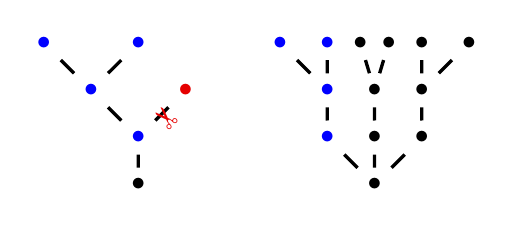
\begin{tikzpicture}[very thick, scale=0.3]
  \node (h1) at (4,0){$\bullet$};
  \node[blue] (h2) at (4,2){$\bullet$};
  \node[blue] (h3) at (2,4){$\bullet$};
  \node[blue] (h4) at (0,6){$\bullet$};
  \node[blue] (h5) at (4,6){$\bullet$};
  \node[red!90!black] (h6) at (6,4){$\bullet$};
  \draw (h1) -- (h2) ;
  \draw (h2) -- (h3) ;
  \draw (h2) -- node[red!90!black,font=\small,sloped,shift={(0.01,-0.075)},rotate=90]{\textbf{\ding{34}}} (h6);
  \draw (h3) -- (h4) ;
  \draw (h3) -- (h5) ;
 
\node (hn1) at (14,0){$\bullet$};
\node[blue] (hn2) at (12,2) {$\bullet$};
\node[blue] (hn3) at (12,4) {$\bullet$};
\node[blue] (hn4) at (10,6){$\bullet$};
  \node[blue] (hn5) at (12,6){$\bullet$};
  \draw (hn1) -- (hn2) ;
  \draw (hn2) -- (hn3) ;
  \draw (hn3) -- (hn4) ;
  \draw (hn3) -- (hn5) ;
\node (hn2b) at (14,2) {$\bullet$};
\node (hn3b) at (14,4) {$\bullet$};
\node (hn4b) at (13.4,6){$\bullet$};
  \node (hn5b) at (14.6,6){$\bullet$};
  \draw (hn1) -- (hn2b) ;
  \draw (hn2b) -- (hn3b) ;
  \draw (hn3b) -- (hn4b) ;
  \draw (hn3b) -- (hn5b) ;
  \node (hn2c) at (16,2) {$\bullet$};
\node (hn3c) at (16,4) {$\bullet$};
\node (hn4c) at (16,6){$\bullet$};
  \node (hn5c) at (18,6){$\bullet$};
  \draw (hn1) -- (hn2c) ;
  \draw (hn2c) -- (hn3c) ;
  \draw (hn3c) -- (hn4c) ;
  \draw (hn3c) -- (hn5c) ;
\end{tikzpicture}

  \caption{Two successive states of a hydra in a battle.  Hercules chopped off the rightmost head of the hydra (red), and the whole left tree except the root node (blue) was copied twice.}
  \label{fig:round}
\end{figure}



 %  \begin{figure}[htb]
% \centering
% \begin{tikzpicture}[very thick, scale=0.3]
% \node (foot) at (10,0) {$\bullet$};
% \node (N1) at (2,2) {$\bullet$};
% \node (N2) at (10,2) {$\bullet$};
% \node (N22) at (7,2) {$\bullet$};
% \node (N3) at (14,2) {$\bullet$};
% \node (N4) at (18,2) {$\Smiley[2][green]$};
% \node (N5) at (0,4) {$\bullet$};
% \node (N6) at (2,5) {$\Smiley[2][green]$};
% \node (N7) at (4,6) {$\Smiley[2][green]$};
% \node (N88) at (7,4) {$\bullet$};
% \node (N8) at (10,4) {$\bullet$};
% \node (N9) at (14,6) {$\Smiley[2][green]$};
% \node (N10) at (0,8) {$\Smiley[2][green]$};
% \node (N11) at (10,7) {$\Smiley[2][green]$};
% \node (N111) at (7,7) {$\Smiley[2][green]$};
% \draw (foot) to [bend left=10] (N1);
% \draw (foot) -- (N2);
% \draw (foot) -- (N22);
% \draw (foot) -- (N3);
% \draw (foot) -- (N4);
% \draw (N1) to  (N5);
% \draw (N1) to   [bend left=10] (N6);
% \draw (N1) to   [bend right=20] (N7);
% \draw (N2) to  (N8);
% \draw (N22) to  (N88);
% \draw (N8) to  (N11);
% \draw (N88) to  (N111);
% \draw (N3) to  (N9);
% \draw (N5) to  (N10);
% \end{tikzpicture}
% \caption{The hydra associated with the ordinal $\omega^{\omega+2}+\omega^\omega \times 2 + \omega + 1$ \label{fig:iota-example}}

% \end{figure}

Kirby and Paris proved the following theorems, applying
combinatorial results about ordinal numbers by Jussi Ketonen and Robert Solovay~\cite{KS81}.

\begin{theorem}
  In the Hydra game, Hercules eventually wins, whichever the strategy of both players:
  choice of a head to chop off, choice of the number of copies.
 \label{kp:thm1}
\end{theorem}

\begin{theorem}
  Theorem~\ref{kp:thm1} cannot be proved in Peano Arithmetic. \label{kp:thm2}
\end{theorem}

The contrast between the simplicity of the statements above and the complexity of their proofs convinced us that it is a good theme for a commented library~\cite{HydraBattles} of formal proofs written for the \coq proof assistant~\cite{Coq}. 

Complex formalizations and proofs are explained in the book.
% an  electronic book~\cite{HydraBook} (PDF document of over 280 pages).
Whenever various reasonable choices exist, we try to present and compare the alternatives.
  For instance, Figures~\ref{fig:Ex42E0} and \ref{fig:Ex42-schutte} show two radically different proofs of the equality
  $\omega+42+\omega^2=\omega^2$. The first one is a simple proof by computation, the second one shows how this equality
  is a consequence of the axioms of the set-theoretic model  by Kurt Schütte~\cite{schutte}. 

This work is also an opportunity to 
 provide concrete examples of formalization and proof techniques: operational type classes, functions defined by  equations, dependently typed functions, etc. It may be also used as a library on ordinal numbers, for instance for proving termination properties.
%
 Prior stages of this project have already been presented at
 JFLA~\cite{PCiota, JFLA2018paper}.
In this paper, we present recent evolutions of the library: new results, interaction with the \community project~\cite{CoqCommunity}, and documentation generated with \alectr~\cite{alectryonpaper, alectryongithub}.

\section{Recent developments}
The 2018 article~\cite{JFLA2018paper} presented a formal proof of the following theorem:

\begin{theorem}
  Let $\mu$ be any ordinal strictly less than $\epsilon_0$.
  There is no function mapping hydras to the segment $[0,\mu)$ that could be used as a measure in proving termination for \emph{any} hydra battle.\label{thm3}
\end{theorem}

Our proof was based on the construction of a battle between Hercules and the hydra where the
number of copies at each round was given by the elimination of an existential quantifier. So, it was mandatory to consider the class of \emph{all} hydra battles, or, equivalently, the class of battles where the hydra choses arbitrarily its number $n$ of copies at every round of the battle.

Unfortunately, the examples  most commonly shown in the literature
(see for instance~\cite{KP82, bauer2008, BauerHydra}) 
assume that the hydra grows $k$ copies at step $k$ of the game, which is incompatible with our proof.
We prove now that Theorem~\ref{thm3} still holds with these typical battles.
%by borrowing new combinatorial results from~\cite{KS81}.
Since we are looking  for a minoration of the length of such battles,
we can work with the following hypotheses and invariants, 
without any loss of generality.
 
 \begin{itemize}
   \item The game starts at an initial step $k=i$, where $i$ is any natural number.
   \item Hercules always chops off the rightmost head of the hydra.
   \item  The hydra is always the tree representation of some ordinal strictly below $\epsilon_0$ in Cantor normal
     form (thus, the rightmost branch is also one of the shortest).
     For instance, Figure~\ref{fig:round} shows the hydras respectively associated with  $\omega^{\omega^2+1}$ and $\omega^{\omega^2}\times 3$.
 \end{itemize}
 
 In mathematical terms, if at step $k\geq i$, the hydra is associated with the ordinal $\alpha$, at step $k+1$ it is associated with
 $\canonseq{\alpha}{k+1}$, \emph{i.e.} the $(k+1)$th element of the canonical sequence of $\alpha$~\cite{KS81}. In the following,  the expression ``the hydra $\alpha$'' is an abbreviation of ``the hydra associated with the ordinal $\alpha$''.
 
 Our new proof of Theorem~\ref{thm3} is based on a systematic study of strictly decreasing sequences of ordinals below $\epsilon_0$, borrowed from Ketonen and Solovay~\cite{KS81}, and the formalization of which is described in detail  in chapters 5 and 6 of~\cite{HydraBook}.

 Besides  Theorem~\ref{thm3}, we study also the number of steps of a battle:
Let $\alpha<\epsilon_0$ be an ordinal. 
We prove that  the number of steps of the battle starting with
$\alpha$ at step $i$ is greater or equal than
$H'_\alpha(i)-i$, where $H'$ is a slight variant of the Hardy hierarchy of rapidly growing functions~\cite{BW85, KS81, Promel2013, Wainer1970}.  The function $H'_\alpha$ is defined by transfinite recursion over $\alpha$ on Figures~\ref{fig:hardy-math}
and~\ref{fig:Hprime}.


\begin{figure}[h]
\begin{align}
  H'_0(i) & = i\\
  H'_\alpha(i) &= H'_{(\canonseq{\alpha}{i+1})}(i)  \quad\textit{if $\alpha$ is a limit ordinal}\\
  H'_{\alpha}(i) &=H'_\beta(i+1) \quad\textit{if $\alpha=\beta+1$}
\end{align}  
  \caption{The $H'$ rapidly growing hierarchy of arithmetical functions}
  \label{fig:hardy-math}
\end{figure}


\begin{figure}[h]
  \centering
  \fbox{
    \begin{minipage}[h]{1.0\linewidth}
 \inputsnippets{Hprime_HprimeDef}     
    \end{minipage}}
 \caption{$H'$ definition with the \texttt{coq-equations}
 plug-in~\cite{sozeau:hal-01671777}}
\label{fig:Hprime}
\end{figure}


Using $H'$s equations as rewrite rules, we can study a concrete example. We take the hydra of figure~\ref{fig:start} and $i=0$ as initial configuration. 
By a sequence of rewritings and inductions, we prove that the number of steps of the considered battle is greater or equal than $2^{2^N}$, where $N=2^{70}-1$.
By comparison with the diagonalized Ackermann function $\lambda\,i.\,A(i,i)$, we prove also that, for $\alpha\geq\omega^\omega$, 
the function computing the length of the battle starting with the hydra $\alpha$ and the initial step $i$ is not primitive recursive.

\begin{figure}[h]
  \centering
  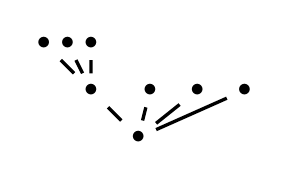
\begin{tikzpicture}[very thick, scale=0.3]
  \node (h1) at (4,0){$\bullet$};
  \node (h2) at (2,2){$\bullet$};
  \node (h3) at (0,4){$\bullet$};
  \node (h4) at (1,4){$\bullet$};
  \node (h5) at (2,4){$\bullet$};
  \node (h6) at (4.5,2){$\bullet$};
  \node (h7) at (6.5,2){$\bullet$};
  \node (h8) at (8.5,2){$\bullet$};
    \draw (h1) -- (h2) ;
    \draw (h2) -- (h3) ;
    \draw (h2) -- (h4) ;
    \draw (h2) -- (h5) ;
    \draw (h1) -- (h6) ;
    \draw (h1) -- (h7) ;
    \draw (h1) -- (h8);
 \end{tikzpicture}

  \caption{The hydra associated with the ordinal $\omega^3+3$}
  \label{fig:start}
\end{figure}




\label{sect:not-pr}

%\TODO[Clément]{Could we use a font with ligatures?}


\section{Integration with \community}

\subsection{Background}

\community is an informal organization run by volunteer Coq users on GitHub that aims to maintain interesting open source Coq projects for the long term and facilitate collaboration among Coq users on documentation, tooling, etc. \community was created in 2018, inspired by the {Elm Community} organization~\cite{zimmermann:tel-02451322}.
%
Such ``Community Package Maintenance Organizations'' exist in many software ecosystems, as they avoid the common problem of an important package becoming unmaintained after its author has moved on to other projects or has disappeared~\cite{zimmermann2021grounded}.

In the case of \coq, this problem is likely even more prevalent than in other ecosystems, as many packages are created by graduate students or researchers for a specific paper and not planned to be maintained for the long term by authors.
%
However, authors are generally open to having someone else who expresses interest in their work take over package maintenance.
%

\community makes it easy to change maintainers by defining a process for transferring or forking an unmaintained package, tooling for setting up good maintenance practices (such as continuous integration), and by making it possible for someone to take over a package without making a long-term commitment (as maintainers who drop out can easily be replaced by some other volunteers).

As of 2021, \community hosts over 50 projects maintained by over 30 volunteers.
%
The hosted projects come from a variety of origins.
%
Some had been maintained in the past by the \coq development team on behalf of the authors, but this meant that only minimal changes required to make the project build with new \coq versions were performed.
%
Some were still maintained by their original authors, but were transferred to enable other users to help out with maintenance and facilitate adoption of best practices on, e.g., continuous integration.
%
Others were simply unmaintained and were revived after their transfer to \community.

Given the objectives of \community, we believe it makes sense to propose a transfer anytime we encounter an interesting Coq project that is insufficiently maintained.
%
After a transfer, the \community maintainers are explicitly allowed to perform large changes and refactorings.
%
This means, for instance, that we can consolidate packages by merging them, or split up a single package into several packages.

\subsection{Integration of primitive recursive functions}

In order to prove formally that the length of the
kind of hydra battles we consider is not given by any primitive recursive function, we chose to use a formalization of primitive recursive functions that was originally part of Russell O'Connor's formal proof of G\"{o}del's first incompleteness theorem~\cite{OConnor05, Goedel}.
For this purpose, and above all in consideration of the scientific interest of this contribution, we decided to host and maintain O'Connor's work in \community.

Since computability is a key topic in computer science teaching and O'Connor's library is a nice illustration of dependently typed programming, we decided to devote a full chapter (chapter 9 of~\cite{HydraBook}) to the formalization of primitive recursive functions, with comments on the definitions and proofs and (counter-)examples and exercises. As part of the writing process, we made the formalization into a new sub-library of the Hydra-battles library, dubbed Ackermann.

\subsection{First steps towards a bridge to \gaia}

The \gaia project by Jos\'e Grimm aimed to formalize mathematics in \coq in the style of Nicolas Bourbaki. The formalization of the first book in the Elements of Mathematics series by Bourbaki, on the theory of sets, was initially described in a technical report in July 2009~\cite{Grimm2009a}. The set-theoretic axioms and basic definitions in \gaia were derived from an earlier development by Carlos Simpson~\cite{Simpson2004,CatsZFCContrib}. Grimm then wrote (and continually updated) technical reports describing the formalization of Bourbaki's two subsequent books~\cite{Grimm2009b,Grimm2016} and additional topics in number theory~\cite{grimm:hal-00911710,Grimm2014}, before he passed away in 2019.

In 2020, members of \community transferred the \gaia source code to GitHub and adapted it for recent releases of the Mathematical Components library, which \gaia heavily relies on. Anonymous volunteers (``collaborators of Nicolas Bourbaki'') then finished the only in-progress proof left by Grimm. At around 155,000 lines of code, \gaia is currently one of the largest maintained open source \coq projects~\cite{Gaia}.

\gaia contains definitions of ordinals in Cantor and Veblen normal form~\cite{grimm:hal-00911710}, adapted from the historical Cantor contribution~\cite{CantorContrib}. The data types for ordinals are essentially defined the same way in \gaia and \Hydras, but they are not identical inside \coq, e.g., due to residing in different modules. Moreover, there are small differences in the implementation of ordinal arithmetic due to different evolutionary paths taken since divergence from the ancestral library.
%
Nevertheless, we were able to establish an initial correspondence between both implementations of ordinals through rewriting lemmas. For instance, we proved that multiplication of ordinals in Cantor normal form in \Hydras refine \gaia's corresponding multiplication operation, and were able to import \gaia's proof of associativity of the multiplication almost for free.

\subsection{Package Genealogy, Dependencies, and Organization}

Both due to its prior stages~\cite{PCiota,JFLA2018paper} and the recent integrations described just above, the current \Hydras \coq code has a complex inheritance. Figure~\ref{fig:genealogy} illustrates the relationships between \Hydras packages and show their ancestry from historical Coq contributions. To indicate the scope and relative sizes of packages, Table~\ref{tbl:loc} breaks down lines of code for each package in the \Hydras galaxy, as reported by the \texttt{coqwc} tool, and lists their repository names in \community and identifiers in the \coq opam package index~\cite{CoqPackageIndex}.

\begin{figure}[ht]
\centering
{\footnotesize
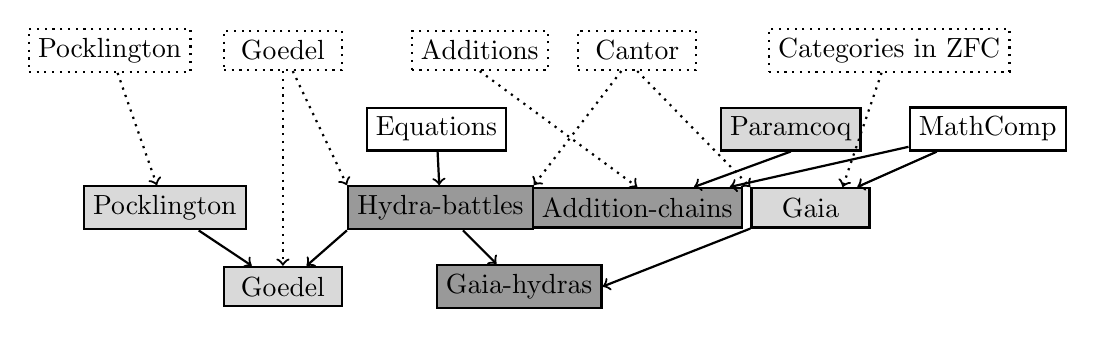
\begin{tikzpicture}[thick]

\begin{scope}[xshift=-6cm]
\node[rectangle, dotted,draw=black,minimum height=0.5cm,minimum width=1.5cm] (goedel) { Goedel };
\node[rectangle, dotted,draw=black,minimum height=0.5cm,minimum width=1.5cm,left of=goedel, node distance=2.2cm] (pock) { Pocklington };
\node[rectangle, dotted,draw=black,minimum height=0.5cm,minimum width=1.5cm,right of=goedel, node distance=2.5cm] (additions) { Additions };
\node[rectangle, dotted,draw=black,minimum height=0.5cm,minimum width=1.5cm,right of=additions, node distance=2cm] (cantor) { Cantor };

\node[rectangle, dotted,draw=black,minimum height=0.5cm,minimum width=1.5cm,right of=cantor, node distance=3.2cm] (cats) { Categories in ZFC };
\end{scope}

\begin{scope}[yshift=-1cm,xshift=0.45cm]
  \node[rectangle, draw=black,fill=gray!30,minimum height=0.5cm,minimum width=1.5cm] (paramcoq) { Paramcoq };
\node[rectangle, draw=black,minimum height=0.5cm,minimum width=1.5cm,right of=paramcoq, node distance=2.5cm] (mathcomp) { MathComp };
\node[rectangle, draw=black,minimum height=0.5cm,minimum width=1.5cm,node distance=2cm,left of=paramcoq, node distance=4.5cm] (equations) { Equations };
\end{scope}

\begin{scope}[yshift=-2cm,xshift=-4cm]
\node[rectangle, draw=black,fill=gray!80,minimum height=0.5cm,minimum width=1.5cm] (hydras) { Hydra-battles };
\node[rectangle, draw=black,fill=gray!30,minimum height=0.5cm,minimum width=1.5cm,left of=hydras, node distance=3.5cm] (pockcc) { Pocklington };
\node[rectangle, draw=black,fill=gray!80,minimum height=0.5cm,minimum width=1.5cm,right of=hydras, node distance=2.5cm] (chains) { Addition-chains };
\node[rectangle, draw=black,fill=gray!30,minimum height=0.5cm,minimum width=1.5cm,right of=chains, node distance=2.2cm] (gaia) { Gaia };
\end{scope}

\begin{scope}[yshift=-3cm,xshift=-6cm]
 \node[rectangle, draw=black,fill=gray!30,minimum height=0.5cm,minimum width=1.5cm] (goedelcc) { Goedel };
 \node[rectangle, draw=black,fill=gray!80,minimum height=0.5cm,minimum width=1.5cm,right of=goedelcc, node distance=3cm] (gaiahydras) { Gaia-hydras };
\end{scope}

\draw[->,dotted] (additions.south) -- (chains.north) ;
\draw[->,dotted] (goedel) -- (goedelcc) ;
\draw[->,dotted] (goedel) -- (hydras.north west) ;
\draw[->,dotted] (cantor) -- (hydras.north east) ;
\draw[->,dotted] (cantor.south) -- (gaia.north west) ;
\draw[->,dotted] (pock) -- (pockcc) ;
\draw[->,dotted] ([xshift=2.1cm]cats) -- (gaia) ;

\draw[->] (hydras) -- (gaiahydras) ;
\draw[->] (hydras.south west) -- (goedelcc) ;
\draw[->] (gaia.south west) -- (gaiahydras.east) ;

\draw[->] (equations) -- (hydras) ;
\draw[->] (mathcomp) -- (gaia) ;
\draw[->] (mathcomp) -- (chains) ;
\draw[->] (paramcoq.south) -- (chains) ;
\draw[->] (pockcc) -- (goedelcc) ;
\end{tikzpicture}
}
\caption{Genealogy and dependencies for \Hydras packages. Dotted boxes represent historical Coq contributions, while regular boxes represent maintained \coq packages. Dark gray packages are maintained in the \Hydras GitHub repository, while light gray packages are maintained in other \community repositories. Dotted lines represent \coq code ancestry, while regular lines represent direct code dependencies.}
  \label{fig:genealogy}
\end{figure}

Before the Ackermann sub-library was moved from the Goedel package repository to the \Hydras repository, the Goedel package had around 7,000 specification LOC and 38,000 proof LOC. Figure~\ref{fig:genealogy} and Table~\ref{tbl:loc} thus reveal that the seemingly large Coq formalization of G\"{o}del's incompleteness theorem can be viewed as a modestly-sized proof on top of general libraries for, on the one hand, first-order logic, primitive recursive functions, and Peano Arithmetic (Ackermann), and on the other hand, prime numbers and their properties (Pocklington).

\begin{table}[ht]
\centering
\footnotesize
\begin{tabular}{llllrr}
\hline
\textbf{Package name} & \textbf{Repository} & \textbf{Index identifier} & \textbf{Version} & \textbf{Spec LOC} & \textbf{Proof LOC}\\
\hline
Pocklington & \href{https://github.com/coq-community/pocklington}{\texttt{pocklington}} & \texttt{coq-pocklington} & \texttt{8.12.0} & 825 & 3,798 \\
Goedel & \href{https://github.com/coq-community/goedel}{\texttt{goedel}} & \texttt{coq-goedel} & \texttt{8.13.0} & 2,799 & 10,762 \\
Gaia & \href{https://github.com/coq-community/gaia}{\texttt{gaia}} & \texttt{coq-gaia} & \texttt{1.12} & 28,850 & 124,839 \\
Hydra-battles & \href{https://github.com/coq-community/hydra-battles}{\texttt{hydra-battles}} & \texttt{coq-hydra-battles} & \texttt{0.5} & 14,368 & 48,385 \\
Addition-chains & \href{https://github.com/coq-community/hydra-battles}{\texttt{hydra-battles}} & \texttt{coq-addition-chains} & \texttt{0.5} & 1,961 & 2,210 \\
Gaia-hydras & \href{https://github.com/coq-community/hydra-battles}{\texttt{hydra-battles}} & \texttt{coq-gaia-hydras} & \texttt{0.5} & 81 & 177 \\
\hline
\end{tabular}
\caption{Current numbers of lines of code for packages in the \Hydras galaxy.}
\label{tbl:loc}
\end{table}

In traditional software development, it is common for packages to continually depend on a large number of packages. In contrast, projects in the Coq ecosystem are often subject to ``dependency aversion'', where maintainers eschew depending on useful packages because it may lead to work in adapting to upstream changes. With \Hydras, we hope to demonstrate that projects with complex dependencies are feasible to manage using recent advances in build management and infrastructure.

% We could already talk a bit of the monorepo structure here, and
% defer some explanations on the tooling to the next section.

\section{Modernizing the build infrastructure}

\subsection{Documentation with \alectr}

The \Hydras book is written in LaTeX, but it makes very frequent references (about once per page, 274 snippets over 281 pages) to parts of the \coq development, showing definitions (Fig.~\ref{fig:Hprime}), computation results (Fig.~\ref{fig:Pow-evalPow17LetIn}), lemmas (Fig.~\ref{fig:Ex42E0}) and parts of  proof scripts (Fig.~\ref{fig:Ex42-schutte}). The order in which these references appear in the book is independent of the structure of our libraries, so we chose to maintain the book as a standalone document, separate from the \coq source code.  This contrasts with the \coqdoc approach, where explanatory prose is embedded within \coq source files (a detailed discussion of different approaches to documenting \coq developments can be found in \cite{alectryonpaper}).

Originally, we copied snippets from \coq sources into LaTeX manually, and recorded and inserted the corresponding outputs manually as well.  This approach is common, but brittle: changes to \coq definitions or lemmas had to be reflected in the book's sources, and we found multiple instances where the book and the \coq development had diverged.
 
We solved this maintenance issue by moving to \alectr, a tool that automatically records \coq proofs~\cite{alectryongithub}.  Instead of copy-pasting fragments into LaTeX, we now embed small LaTeX files automatically generated by \alectr from our \coq development.  Our build system guarantees that these LaTeX snippets are always up-to-date and consistent with the code (and, by comparing these snippets across releases of \coq or versions of \Hydras, we can easily spot unexpected changes).

Importing snippets into a LaTeX document was not one of the original use cases of Alectryon. Firstly, the original Alectryon did not have support for exporting to LaTeX. Secondly, it was geared towards documenting individual source files, where code and prose are interleaved within the same file. In this style, the code is documented in the same order as it is compiled.
We extended \alectr to support our needs by implementing a LaTeX backend, and by programming it to generate individual snippet files, one per \texttt{snippet} comment block.  The later part was straightforward: all it took was to build a custom \alectr \textit{driver}, a small (about 100 lines) Python program that leverages most of the \alectr toolchain but defines a custom frontend that understands our snippet annotations (and otherwise exposes the exact same command line as \alectr).

Once the infrastructure was in place, the transition happened gradually, over a few weeks: for each snippet of \coq code that was in the book, we had to take the following steps:

\begin{enumerate}
\item Mark the snippet in the \coq sources (we use special comments \texttt{(* begin snippet \textit{name} *)} … \texttt{(* end snippet \textit{name} *)})
\item Configure output display, using special \alectr annotations to configure what should be shown (only the inputs, inputs and outputs, some steps of the proof but not all, some proof states at key moments in a proof, etc.)
\item Replace the copy-pasted inputs and output in LaTeX with an \texttt{input} command.
\end{enumerate}

   \begin{figure}[h]
     \centering
     \fbox{
       \begin{minipage}[h]{1.0\linewidth}
         \inputsnippets{Pow_evalPow17LetIn}
       \end{minipage}}
  \caption{\label{fig:Pow-evalPow17LetIn}Automatically capturing the output of computations}
\end{figure}


  \begin{figure}[h]
    \centering
    \fbox{
      \begin{minipage}[h]{1.0\linewidth}
        \inputsnippets{E0_Ex42}
      \end{minipage}}
    \caption{A simple proof by computation}
    \label{fig:Ex42E0}
  \end{figure}



%\afterpage{\clearpage}

 


\begin{figure}[th]
  \centering
  
  

\fbox{\begin{minipage}[h]{1.0\linewidth}
  Let us prove again the equality $\omega+42+\omega^2= \omega^2$. We recall that $\omega^2$ is an abbreviation of $\phi_0(2)$,
\emph{i.e} the third  additive principal ordinal, and that \texttt{F} is a notation for the coercion which maps natural numbers to ordinals.

\inputsnippets{Schutte_Ex42a}


Our proof is very different from the computational proof of
Figure~\ref{fig:Ex42E0}.
By definition of additive principal ordinals, 
it suffices to prove the inequality $\omega+42< \phi_0(2)$.

\inputsnippets{Schutte_Ex42b}

Since the set \textit{AP} of additive principals  is closed under addition
(by Lemma \textit{AP\_plus\_closed}), it suffices to prove the inequalities $\omega<\omega^2$ and $42<\omega^2$.

\inputsnippets{Schutte_Ex42d, %to remove if short paper
  Schutte_Ex42c, Schutte_Ex42e}

\end{minipage}
}
\caption{A proof interleaved with text (from the book)}
  \label{fig:Ex42-schutte}
\end{figure}


\subsection{Technologies supporting the monorepo structure}

A monorepo (shorthand for monolithic repository) is a version control repository containing multiple independent or related packages.
%
Monorepos have gained increasing popularity following experiences in large companies such as Google, but are also used at a smaller scale for managing open source projects.
%
They are known to simplify the management of dependencies, making cross-packages changes, and refactorings~\cite{brito2018monorepos}.

%
One of the few early uses of monorepos in the Coq ecosystem was for the Mathematical Components library~\cite{MCB}, whose maintainers developed a custom build infrastructure to check multiple packages on each commit.
%
In light of that recent tooling improvements have made monorepo use easier, we chose to use an explicit monorepo structure for \Hydras in \community. Other \community projects have since adopted a similar structure.

In the context of \Hydras, we rely on the following tools.

\paragraph{The Dune build system~\cite{dune}.}
Dune was originally designed to build OCaml projects, but was recently extended to support Coq. Dune allows building packages contained in a single source tree separately, which is essential to be able to publish the different libraries contained in a single repository as separate (opam) packages to the Coq package index.

However, Dune is still inconvenient for local IDE-based Coq code development and does not yet support building Coqdoc files.
%
Therefore, we still support building the whole project using \make via the \coqmakefile tool bundled with \coq, and we rely on this build system in our documentation generation pipeline.
%
We expect to migrate fully to Dune as soon as these limitations are lifted.

\paragraph{The Docker-Coq-Action~\cite{martindorel2020dockercoq}.}
This GitHub Action provides a very simple way of setting up Continuous Integration (CI) for a Coq project with an opam file.
%
At the current time, we rely on it, together with the mathcomp Docker images~\cite{mathcompdocker}, to test our two main libraries, Hydra-battles and Addition-chains, with multiple versions of Coq.

\paragraph{The Coq Nix Toolbox~\cite{cohen:hal-03366644}.}
This toolbox, based on the Nix package manager, provides an alternative way of setting up CI for a Coq project (also relying on GitHub Actions).
%
We use this Nix-based CI for several things.

\begin{enumerate}
\item To test the build of the project (as a single unit) with \coqmakefile (whereas the Docker-based CI relies on the opam packages, which use Dune to build the libraries contained in the project).

\item To generate the documentation of the project (book in PDF format and \coqdoc HTML pages) by relying on the output of the \coqmakefile build.

\item To test the bridge to the Gaia library, because the Nix-based CI supports out-of-the-box caching of build dependencies.
%
Given that Gaia takes more than 5 minutes to build, this build is only done once, then reused at each new run of the CI.

\item To test compatibility with the Goedel library, which was made to depend on the Hydra-battles library since the Ackermann sub-library was moved from the former to the latter.
%
For this, we rely on the fact that the Coq Nix Toolbox has native support for generating a CI configuration that includes reverse dependency compatibility testing.
\end{enumerate}

The artifacts of the Nix builds are stored in the \community binary cache on Cachix~\cite{cachix}.
%
This means that a given version never has to be built twice and Continuous Integration can be almost instantaneous when no change has been made (e.g., after merging a pull request).

By relying on two different technologies for CI, we are able to fit a larger range of use cases, while also providing more assurance that the project does build correctly in a variety of configurations.
%
Given that the two technologies are well maintained (within \community), relying on both does not incur a significant cost, compared to the benefits they provide.

\section{Comparison of \Hydras with other Coq books}

We believe that Coq books can broadly be divided into two categories:
\begin{itemize}
\item \emph{Executable textbooks} that are in effect large, well-commented Coq programs from which other representations of the material (HTML, PDF) are derived using tools.
\item \emph{Traditional textbooks} generated from documentation languages such as LaTeX that are accompanied by standalone Coq formalizations and/or code snippets.
\end{itemize}
Table~\ref{tbl:books} shows a category breakdown for what we believe are the most prominent Coq books in English. Note that several traditional books, such as Coq'Art~\cite{BC04}, used custom tools during their writing process to keep code snippets synchronized with Coq. However, once a book is published, the accompanying code generally takes on a life of its own~\cite{CoqArtCommunity} and may come to substantially diverge from the book.

\begin{table}
  \centering
  \footnotesize
  \begin{tabular}{lll}
  \hline
  \textbf{Title} & \textbf{Year} & \textbf{Category}\\
  \hline
  Coq'Art~\cite{BC04} & 2004 & Traditional\\
  Software Foundations~\cite{SF} & 2007 & Executable\\
  Certified Programming with Dependent Types~\cite{chlipalacpdt2011} & 2011 &  Executable\\
  Program Logics for Certified Compilers~\cite{Appel2014} & 2014 & Traditional\\
  Programs and Proofs~\cite{Sergey:PnP} & 2014 & Executable\\
  Formal Reasoning About Programs~\cite{Chlipala2017} & 2017 & Traditional\\
  Computer Arithmetic and Formal Proofs~\cite{Boldo2017} & 2017 & Traditional\\
  Mathematical Components~\cite{MCB} & 2018 & Traditional\\
  \hline
  \end{tabular}
  \caption{Coq book categorization.}
  \label{tbl:books}
\end{table}

We believe the \Hydras electronic book has found an attractive set of tradeoffs between the properties of executable books and traditional books. Specifically, in an executable book, the proof assistant language places limits on the structure. For example, Coq may not permit repeating a definition from another file verbatim, since the definition uses variables that are not present in the current context. Thanks to our \alectr based toolchain, the \Hydras book can include ``live'' code fragments at any point in the text. And in contrast to traditional books, we validate the consistency of code fragments during every build of the electronic book. On the one hand, we follow executable books in providing ``continuous delivery'' of new revisions at a high pace. But on the other hand, we also aim to make regular timestamped versions compatible with specific versions of Coq, akin to new editions of traditional books.

Due to our reliance on LaTeX for writing the book, obtaining a book representation in HTML is more cumbersome than for executable books such as Software Foundations~\cite{SF} and Certified Programming with Dependent Types~\cite{chlipalacpdt2011}. Currently, we generate the Coq code documentation in HTML form separately from the book.

\section{Conclusion and perspectives}


\Hydras wants to provide a connection between scientific literature (\emph{e.g.},~\cite{KP82, KS81, schutte}) and proof assistant technology. For the mathematician, it can give a concrete view of the mathematical content, not only through full proofs, but also through illuminating computations: examples, functions associated with constructive proofs, etc. For the \coq learner, it provides a consistent set of examples,
allowing to present and compare various formalization and proving techniques. %It may be also used as a library, through opam packages.
It is also a medium sized library (more than 50,000 LOC), dependent on various tools and libraries of the \coq ecosystem, which may be also used to experiment with new maintenance techniques of the code and its documentation. To facilitate easy dissemination and reuse, all code and documentation is available under the permissive MIT license.





%\TODO{General Conclusion}



%\subsection{Perspectives}

%\subsection{Further extensions}

We plan to extend \Hydras in two main directions. Firstly, we plan to bridge the combinatorial results of \Hydras and the set-theoretic content of \gaia, enabling the transfer of many interesting theorems between the two packages. Secondly, we aim to write a formal proof in \coq of the original statement of Theorem~\ref{kp:thm2}, using O'Connor's formalization of Peano Arithmetic~\cite{Goedel}.
%
Moreover, \Hydras is not limited to the study of ordinal numbers and applications.
We are also developing a package about efficient exponentiation
algorithms, and aim to eventually include new topics. We invite new collaborators to join us in our efforts.

\section*{Acknowledgments}
\label{sect:acks}
We thank the anonymous reviewers for their comments, and we are grateful to the original authors and current maintainers of the Coq packages we use and depend on: José Grimm (Gaia), Russell O'Connor (Goedel), Matthieu Sozeau (Equations), the Mathematical Components team, Marc Lasson and Chantal Keller (Paramcoq), and the authors and maintainers of \coq and its associated tools.


\label{sect:bib}
\bibliographystyle{plain}
%\bibliographystyle{alpha}
%\bibliographystyle{unsrt}
%\bibliographystyle{abbrv}
% easychair.tex,v 3.5 2017/03/15

\documentclass{easychair}
%\documentclass[EPiC]{easychair}
%\documentclass[EPiCempty]{easychair}
%\documentclass[debug]{easychair}
%\documentclass[verbose]{easychair}
%\documentclass[notimes]{easychair}
%\documentclass[withtimes]{easychair}
%\documentclass[a4paper]{easychair}
%\documentclass[letterpaper]{easychair}

\usepackage{doc}
\usepackage{tikz}
\usepackage{tikzsymbols}
\usepackage{pifont}
\newtheorem{theorem}{Theorem}
\usetikzlibrary{arrows}

%\usepackage[firstpageonly=false, color={[gray]{0.5}},
%   scale=2.0, text=DRAFT]{draftwatermark}
% -------------------------------
%%%% For Alectryon

\usepackage{texments}
%%% for movies by alectryon
\usepackage{alectryon}
\usepackage{pygments}
%%% One hypothesis per line 
\makeatletter
\renewcommand{\alectryon@hyps@sep}{\alectryon@nl}
\makeatother

%%% \snippets{A,B,C,…} inputs a series of snippets as one block (with \itemsep
%%% between them).  A, B, C should be paths to files in snippets/.
\usepackage{etoolbox}
\makeatletter
\newcommand{\inputsnippets}[1]
  {{\setlength{\itemsep}{1pt}\setlength{\parsep}{0pt}% Adjust spacing
    \alectryon@copymacros\begin{io}
      \forcsvlist{\item\@inputsnippet}{#1}
    \end{io}}}
\let\input@old\input % Save definition of \input
\newcommand{\@inputsnippet}[1]
  {{\renewenvironment{alectryon}{}{}% Skip \begin{alectryon} included in snippet
    \input@old{#1}}}
\makeatother

%---------------------------- 
\newcommand{\canonseq}[2]{\mbox{$\{#1\}(#2)$}}

\usepackage{varioref}
\newtheorem{todo}{To do}
\usepackage{amsfonts, afterpage}
\usepackage{xspace}

\newcommand{\easychair}{\textsf{easychair}}
\newcommand{\miktex}{MiK{\TeX}}
\newcommand{\texniccenter}{{\TeX}nicCenter}
\newcommand{\makefile}{\texttt{Makefile}}
\newcommand{\latexeditor}{LEd}

%\makeindex

%% Front Matter
%%
% Regular title as in the article class.
%
% \title{Hydras,  Ordinals \& Co.   \\
%   A library in Coq of entertaining formal mathematics}

\title{Hydras \& Co.: Formalized mathematics in Coq\\
 for inspiration and entertainment
}

\author{
Pierre Castéran \inst{1}
\and
    Jérémy Damour \inst{2}
\and
Karl Palmskog \inst{3}
\and Clément Pit-Claudel \inst{4}
\and Théo Zimmermann \inst{5}
}


\institute{
Univ. Bordeaux, CNRS, Bordeaux INP, LaBRI, UMR 5800, F-33400 Talence, France  %\\
 % \email{pierre.casteran@labri.fr}
\and
Univ. de Paris, F-75013 Paris, France
\and
KTH Royal Institute of Technology, Stockholm, Sweden
\and
MIT CSAIL, Cambridge, Massachusetts, USA
\and
Inria, Univ. de Paris, CNRS, IRIF, UMR 8243, F-75013 Paris, France
}



\authorrunning{Castéran, Damour, Palmskog, Pit-Claudel and Zimmermann}

\titlerunning{\Hydras}

\newcommand{\TODO}[2][]{[\textcolor{red}{TODO (#1):} \emph{#2}]}
\newcommand{\coq}{Coq\xspace}
\newcommand{\coqdoc}{Coqdoc\xspace}
\newcommand{\coqmakefile}{\texttt{coq\_makefile}\xspace}
\newcommand{\community}{Coq-community\xspace}
\newcommand{\gaia}{Gaia\xspace}
\newcommand{\alectr}{Alectryon\xspace}
\newcommand{\equations}{Equations\xspace}
\newcommand{\Hydras}{Hydras \& Co$\text.$\xspace}
\newcommand{\make}{\texttt{make}\xspace}
%\newcommand{\Hydras}{Hydra-battles\xspace}

\begin{document}

\maketitle


\begin{abstract}
  \Hydras is a collaborative library of discrete mathematics for the
  \coq proof assistant, developed as part of the \community organization
  on GitHub. The Coq code is accompanied
  by an electronic book, generated with the help of the \alectr
  literate proving tool. We present the evolution of the mathematical
  contents of the library since former presentations at JFLA meetings.
  Then, we describe how the structure of the project is determined
  by two requirements which must be continuously satisfied.
  First, the Coq code needs to be compatible with its ever-evolving
  dependencies (the Coq proof assistant and several Coq packages both from
  inside and outside \community) and reverse dependencies (\community
  projects that depend on it). Second, the book needs to be consistent
  with the Coq code, which undergoes frequent changes to improve
  structure and include new material. We believe \Hydras demonstrates
  that books on formalized mathematics are not limited to
  providing exposition of theories and reasoning techniques---they
  can also provide inspiration and entertainment that transcend educational goals.
\end{abstract}


% \setcounter{tocdepth}{2}
% {\small
% \tableofcontents}


%------------------------------------------------------------------------------
\section{Introduction}
\label{sect:introduction}

\subsection{Background}

Libraries of formalized mathematics based on proof assistants, such as \coq, Lean, and Isabelle/HOL, are continually growing in size and scope.
For example, Mathlib for Lean and the core set of projects in the Mathematical Components family for Coq both amount to hundreds of thousands of lines of code (LOC) and tens of thousands of definitions and theorems~\cite{Nie2020a, Mathlib}. However, after a key mathematical definition or result is added to a library, it must be \emph{documented and maintained}~\cite{vanDoorn2020,alectryonpaper}.

Maintenance includes not only adaptation to changes in new proof assistant versions, but also reorganization to accommodate new contributions. Documentation is usually two-fold: \emph{source code comments} that describe specific definitions and results in-line and \emph{books} that carefully introduce the library and its idioms~\cite{MCB,TheoremProvingLean4}. The former tends to be terse and dense and serves experienced users, while the latter is more long-winded and exhaustive and serves beginners. As a library changes and expands, all its documentation needs to be made consistent and complete. Authors use many techniques, including literate programming~\cite{Knuth1984} and custom tools, to pretty-print and check source code snippets and generate proof assistant output.

While books that document proof assistant libraries are valuable to beginners, the purpose of recently published books is mainly instrumental, i.e., to teach a certain topic or technique. We believe that books and libraries can instead become \emph{ends in themselves}---not just sources of exposition and learning, but also sources of inspiration and entertainment.

\subsection{Vision}
The \Hydras project, part of \community on GitHub~\cite{CoqCommunity}, aims to be an experimental platform for the collaborative development of documented libraries of formal proofs. \community is a community organization that the first and last authors founded in 2018 with two goals in mind: providing a solution for the long-term maintenance of interesting open source \coq packages, and working collaboratively on documentation projects. The \Hydras project demonstrates that these two goals are not independent: interesting \coq packages can become the basis for new documentation.
%
This umbrella project now includes evolved versions of the former Cantor and Additions libraries~\cite{CantorContrib,AdditionsContrib} (under the new names of Hydra-battles and Addition-chains), the Ackermann sub-library extracted from Russel O'Connor's Goedel library~\cite{OConnor05, Goedel}, and a bridge to the \gaia library by José Grimm~\cite{Gaia,grimm:hal-00911710}.
%
By following this approach of commenting interesting \coq packages, we provide new documentation content that contributes to the diversity of the thriving \coq ecosystem.

We call on the \coq users in the JFLA community and beyond to come and join us in this effort, by bringing new interesting projects which are worth presenting to \coq learners, \emph{a.k.a.} \coq users, and guiding them in their exploration.
%
We also always have project ideas to extend further our explorations and anyone is welcome to join the team by sending small or larger contributions through pull requests.
%
The current state of the project is already the result of such evolutions after several of us contributed project solutions and new proposals to the initial version of the first author.

Futhermore, contrary to traditionally published books, the ``book'' that forms part of this project is intended to be forever evolving. As new \coq formalization patterns and proof techniques appear, the book can be adapted to demonstrate their use (in case they fit well with our applications).
%
By using modern maintenance techniques such as continuous integration and deployment, we can ensure that this documentation stays up to date with the latest \coq releases. With \alectr~\cite{alectryonpaper, alectryongithub}, we ensure that code and documentation are always in sync.

\subsection{Hydra games}

We chose to build our library and book on two simple themes which allow many variations: computing powers in a monoid, and Kirby and Paris' hydra battles. In the interest of space, we will only present the second theme in this paper.


Hydra games (also known as \emph{Hydra battles}) appear in an article published in 1982 by two mathematicians, 
Laurie Kirby and Jeff Paris: \emph{Accessible Independence Results for Peano Arithmetic}~\cite{KP82}.
This article describes a game between two players: Hercules and a hydra.
A short description of the game  can be found in~\cite{bauer2008, KP82, JFLA2018paper}. One can also play with
Andrej Bauer's simulator~\cite{BauerHydra}.
In a few words:
\begin{itemize}
\item A hydra is a finite tree, traditionally presented with the root at the bottom, the leaves of which are called \emph{heads}
  (Figure~\ref{fig:round}).
\item At every round, Hercules chops off one head of the hydra. If the head is at a distance greater than 1 from the root,
  then some sub-tree $h$ of the hydra is copied a certain amount $n$ of times. The number $n$ of copies and the sub-tree $h$ may depend on the considered variant of the game
  and the time elapsed since the beginning of the fight.
  Figure~\ref{fig:round} shows an example with $n=2$.
\end{itemize}



\begin{figure}[h]
  \centering
  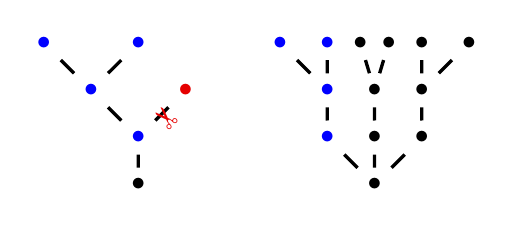
\begin{tikzpicture}[very thick, scale=0.3]
  \node (h1) at (4,0){$\bullet$};
  \node[blue] (h2) at (4,2){$\bullet$};
  \node[blue] (h3) at (2,4){$\bullet$};
  \node[blue] (h4) at (0,6){$\bullet$};
  \node[blue] (h5) at (4,6){$\bullet$};
  \node[red!90!black] (h6) at (6,4){$\bullet$};
  \draw (h1) -- (h2) ;
  \draw (h2) -- (h3) ;
  \draw (h2) -- node[red!90!black,font=\small,sloped,shift={(0.01,-0.075)},rotate=90]{\textbf{\ding{34}}} (h6);
  \draw (h3) -- (h4) ;
  \draw (h3) -- (h5) ;
 
\node (hn1) at (14,0){$\bullet$};
\node[blue] (hn2) at (12,2) {$\bullet$};
\node[blue] (hn3) at (12,4) {$\bullet$};
\node[blue] (hn4) at (10,6){$\bullet$};
  \node[blue] (hn5) at (12,6){$\bullet$};
  \draw (hn1) -- (hn2) ;
  \draw (hn2) -- (hn3) ;
  \draw (hn3) -- (hn4) ;
  \draw (hn3) -- (hn5) ;
\node (hn2b) at (14,2) {$\bullet$};
\node (hn3b) at (14,4) {$\bullet$};
\node (hn4b) at (13.4,6){$\bullet$};
  \node (hn5b) at (14.6,6){$\bullet$};
  \draw (hn1) -- (hn2b) ;
  \draw (hn2b) -- (hn3b) ;
  \draw (hn3b) -- (hn4b) ;
  \draw (hn3b) -- (hn5b) ;
  \node (hn2c) at (16,2) {$\bullet$};
\node (hn3c) at (16,4) {$\bullet$};
\node (hn4c) at (16,6){$\bullet$};
  \node (hn5c) at (18,6){$\bullet$};
  \draw (hn1) -- (hn2c) ;
  \draw (hn2c) -- (hn3c) ;
  \draw (hn3c) -- (hn4c) ;
  \draw (hn3c) -- (hn5c) ;
\end{tikzpicture}

  \caption{Two successive states of a hydra in a battle.  Hercules chopped off the rightmost head of the hydra (red), and the whole left tree except the root node (blue) was copied twice.}
  \label{fig:round}
\end{figure}



 %  \begin{figure}[htb]
% \centering
% \begin{tikzpicture}[very thick, scale=0.3]
% \node (foot) at (10,0) {$\bullet$};
% \node (N1) at (2,2) {$\bullet$};
% \node (N2) at (10,2) {$\bullet$};
% \node (N22) at (7,2) {$\bullet$};
% \node (N3) at (14,2) {$\bullet$};
% \node (N4) at (18,2) {$\Smiley[2][green]$};
% \node (N5) at (0,4) {$\bullet$};
% \node (N6) at (2,5) {$\Smiley[2][green]$};
% \node (N7) at (4,6) {$\Smiley[2][green]$};
% \node (N88) at (7,4) {$\bullet$};
% \node (N8) at (10,4) {$\bullet$};
% \node (N9) at (14,6) {$\Smiley[2][green]$};
% \node (N10) at (0,8) {$\Smiley[2][green]$};
% \node (N11) at (10,7) {$\Smiley[2][green]$};
% \node (N111) at (7,7) {$\Smiley[2][green]$};
% \draw (foot) to [bend left=10] (N1);
% \draw (foot) -- (N2);
% \draw (foot) -- (N22);
% \draw (foot) -- (N3);
% \draw (foot) -- (N4);
% \draw (N1) to  (N5);
% \draw (N1) to   [bend left=10] (N6);
% \draw (N1) to   [bend right=20] (N7);
% \draw (N2) to  (N8);
% \draw (N22) to  (N88);
% \draw (N8) to  (N11);
% \draw (N88) to  (N111);
% \draw (N3) to  (N9);
% \draw (N5) to  (N10);
% \end{tikzpicture}
% \caption{The hydra associated with the ordinal $\omega^{\omega+2}+\omega^\omega \times 2 + \omega + 1$ \label{fig:iota-example}}

% \end{figure}

Kirby and Paris proved the following theorems, applying
combinatorial results about ordinal numbers by Jussi Ketonen and Robert Solovay~\cite{KS81}.

\begin{theorem}
  In the Hydra game, Hercules eventually wins, whichever the strategy of both players:
  choice of a head to chop off, choice of the number of copies.
 \label{kp:thm1}
\end{theorem}

\begin{theorem}
  Theorem~\ref{kp:thm1} cannot be proved in Peano Arithmetic. \label{kp:thm2}
\end{theorem}

The contrast between the simplicity of the statements above and the complexity of their proofs convinced us that it is a good theme for a commented library~\cite{HydraBattles} of formal proofs written for the \coq proof assistant~\cite{Coq}. 

Complex formalizations and proofs are explained in the book.
% an  electronic book~\cite{HydraBook} (PDF document of over 280 pages).
Whenever various reasonable choices exist, we try to present and compare the alternatives.
  For instance, Figures~\ref{fig:Ex42E0} and \ref{fig:Ex42-schutte} show two radically different proofs of the equality
  $\omega+42+\omega^2=\omega^2$. The first one is a simple proof by computation, the second one shows how this equality
  is a consequence of the axioms of the set-theoretic model  by Kurt Schütte~\cite{schutte}. 

This work is also an opportunity to 
 provide concrete examples of formalization and proof techniques: operational type classes, functions defined by  equations, dependently typed functions, etc. It may be also used as a library on ordinal numbers, for instance for proving termination properties.
%
 Prior stages of this project have already been presented at
 JFLA~\cite{PCiota, JFLA2018paper}.
In this paper, we present recent evolutions of the library: new results, interaction with the \community project~\cite{CoqCommunity}, and documentation generated with \alectr~\cite{alectryonpaper, alectryongithub}.

\section{Recent developments}
The 2018 article~\cite{JFLA2018paper} presented a formal proof of the following theorem:

\begin{theorem}
  Let $\mu$ be any ordinal strictly less than $\epsilon_0$.
  There is no function mapping hydras to the segment $[0,\mu)$ that could be used as a measure in proving termination for \emph{any} hydra battle.\label{thm3}
\end{theorem}

Our proof was based on the construction of a battle between Hercules and the hydra where the
number of copies at each round was given by the elimination of an existential quantifier. So, it was mandatory to consider the class of \emph{all} hydra battles, or, equivalently, the class of battles where the hydra choses arbitrarily its number $n$ of copies at every round of the battle.

Unfortunately, the examples  most commonly shown in the literature
(see for instance~\cite{KP82, bauer2008, BauerHydra}) 
assume that the hydra grows $k$ copies at step $k$ of the game, which is incompatible with our proof.
We prove now that Theorem~\ref{thm3} still holds with these typical battles.
%by borrowing new combinatorial results from~\cite{KS81}.
Since we are looking  for a minoration of the length of such battles,
we can work with the following hypotheses and invariants, 
without any loss of generality.
 
 \begin{itemize}
   \item The game starts at an initial step $k=i$, where $i$ is any natural number.
   \item Hercules always chops off the rightmost head of the hydra.
   \item  The hydra is always the tree representation of some ordinal strictly below $\epsilon_0$ in Cantor normal
     form (thus, the rightmost branch is also one of the shortest).
     For instance, Figure~\ref{fig:round} shows the hydras respectively associated with  $\omega^{\omega^2+1}$ and $\omega^{\omega^2}\times 3$.
 \end{itemize}
 
 In mathematical terms, if at step $k\geq i$, the hydra is associated with the ordinal $\alpha$, at step $k+1$ it is associated with
 $\canonseq{\alpha}{k+1}$, \emph{i.e.} the $(k+1)$th element of the canonical sequence of $\alpha$~\cite{KS81}. In the following,  the expression ``the hydra $\alpha$'' is an abbreviation of ``the hydra associated with the ordinal $\alpha$''.
 
 Our new proof of Theorem~\ref{thm3} is based on a systematic study of strictly decreasing sequences of ordinals below $\epsilon_0$, borrowed from Ketonen and Solovay~\cite{KS81}, and the formalization of which is described in detail  in chapters 5 and 6 of~\cite{HydraBook}.

 Besides  Theorem~\ref{thm3}, we study also the number of steps of a battle:
Let $\alpha<\epsilon_0$ be an ordinal. 
We prove that  the number of steps of the battle starting with
$\alpha$ at step $i$ is greater or equal than
$H'_\alpha(i)-i$, where $H'$ is a slight variant of the Hardy hierarchy of rapidly growing functions~\cite{BW85, KS81, Promel2013, Wainer1970}.  The function $H'_\alpha$ is defined by transfinite recursion over $\alpha$ on Figures~\ref{fig:hardy-math}
and~\ref{fig:Hprime}.


\begin{figure}[h]
\begin{align}
  H'_0(i) & = i\\
  H'_\alpha(i) &= H'_{(\canonseq{\alpha}{i+1})}(i)  \quad\textit{if $\alpha$ is a limit ordinal}\\
  H'_{\alpha}(i) &=H'_\beta(i+1) \quad\textit{if $\alpha=\beta+1$}
\end{align}  
  \caption{The $H'$ rapidly growing hierarchy of arithmetical functions}
  \label{fig:hardy-math}
\end{figure}


\begin{figure}[h]
  \centering
  \fbox{
    \begin{minipage}[h]{1.0\linewidth}
 \inputsnippets{Hprime_HprimeDef}     
    \end{minipage}}
 \caption{$H'$ definition with the \texttt{coq-equations}
 plug-in~\cite{sozeau:hal-01671777}}
\label{fig:Hprime}
\end{figure}


Using $H'$s equations as rewrite rules, we can study a concrete example. We take the hydra of figure~\ref{fig:start} and $i=0$ as initial configuration. 
By a sequence of rewritings and inductions, we prove that the number of steps of the considered battle is greater or equal than $2^{2^N}$, where $N=2^{70}-1$.
By comparison with the diagonalized Ackermann function $\lambda\,i.\,A(i,i)$, we prove also that, for $\alpha\geq\omega^\omega$, 
the function computing the length of the battle starting with the hydra $\alpha$ and the initial step $i$ is not primitive recursive.

\begin{figure}[h]
  \centering
  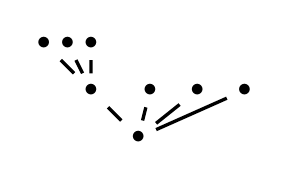
\begin{tikzpicture}[very thick, scale=0.3]
  \node (h1) at (4,0){$\bullet$};
  \node (h2) at (2,2){$\bullet$};
  \node (h3) at (0,4){$\bullet$};
  \node (h4) at (1,4){$\bullet$};
  \node (h5) at (2,4){$\bullet$};
  \node (h6) at (4.5,2){$\bullet$};
  \node (h7) at (6.5,2){$\bullet$};
  \node (h8) at (8.5,2){$\bullet$};
    \draw (h1) -- (h2) ;
    \draw (h2) -- (h3) ;
    \draw (h2) -- (h4) ;
    \draw (h2) -- (h5) ;
    \draw (h1) -- (h6) ;
    \draw (h1) -- (h7) ;
    \draw (h1) -- (h8);
 \end{tikzpicture}

  \caption{The hydra associated with the ordinal $\omega^3+3$}
  \label{fig:start}
\end{figure}




\label{sect:not-pr}

%\TODO[Clément]{Could we use a font with ligatures?}


\section{Integration with \community}

\subsection{Background}

\community is an informal organization run by volunteer Coq users on GitHub that aims to maintain interesting open source Coq projects for the long term and facilitate collaboration among Coq users on documentation, tooling, etc. \community was created in 2018, inspired by the {Elm Community} organization~\cite{zimmermann:tel-02451322}.
%
Such ``Community Package Maintenance Organizations'' exist in many software ecosystems, as they avoid the common problem of an important package becoming unmaintained after its author has moved on to other projects or has disappeared~\cite{zimmermann2021grounded}.

In the case of \coq, this problem is likely even more prevalent than in other ecosystems, as many packages are created by graduate students or researchers for a specific paper and not planned to be maintained for the long term by authors.
%
However, authors are generally open to having someone else who expresses interest in their work take over package maintenance.
%

\community makes it easy to change maintainers by defining a process for transferring or forking an unmaintained package, tooling for setting up good maintenance practices (such as continuous integration), and by making it possible for someone to take over a package without making a long-term commitment (as maintainers who drop out can easily be replaced by some other volunteers).

As of 2021, \community hosts over 50 projects maintained by over 30 volunteers.
%
The hosted projects come from a variety of origins.
%
Some had been maintained in the past by the \coq development team on behalf of the authors, but this meant that only minimal changes required to make the project build with new \coq versions were performed.
%
Some were still maintained by their original authors, but were transferred to enable other users to help out with maintenance and facilitate adoption of best practices on, e.g., continuous integration.
%
Others were simply unmaintained and were revived after their transfer to \community.

Given the objectives of \community, we believe it makes sense to propose a transfer anytime we encounter an interesting Coq project that is insufficiently maintained.
%
After a transfer, the \community maintainers are explicitly allowed to perform large changes and refactorings.
%
This means, for instance, that we can consolidate packages by merging them, or split up a single package into several packages.

\subsection{Integration of primitive recursive functions}

In order to prove formally that the length of the
kind of hydra battles we consider is not given by any primitive recursive function, we chose to use a formalization of primitive recursive functions that was originally part of Russell O'Connor's formal proof of G\"{o}del's first incompleteness theorem~\cite{OConnor05, Goedel}.
For this purpose, and above all in consideration of the scientific interest of this contribution, we decided to host and maintain O'Connor's work in \community.

Since computability is a key topic in computer science teaching and O'Connor's library is a nice illustration of dependently typed programming, we decided to devote a full chapter (chapter 9 of~\cite{HydraBook}) to the formalization of primitive recursive functions, with comments on the definitions and proofs and (counter-)examples and exercises. As part of the writing process, we made the formalization into a new sub-library of the Hydra-battles library, dubbed Ackermann.

\subsection{Towards a bridge to \gaia}

The \gaia project by Jos\'e Grimm aimed to formalize mathematics in \coq in the style of Nicolas Bourbaki. The formalization of the first book in the Elements of Mathematics series by Bourbaki, on the theory of sets, was initially described in a technical report in July 2009~\cite{Grimm2009a}. The set-theoretic axioms and basic definitions in \gaia were derived from an earlier development by Carlos Simpson~\cite{Simpson2004,CatsZFCContrib}. Grimm then wrote (and continually updated) technical reports describing the formalization of Bourbaki's two subsequent books~\cite{Grimm2009b,Grimm2016} and additional topics in number theory~\cite{grimm:hal-00911710,Grimm2014}, before he passed away in 2019.

In 2020, members of \community transferred the \gaia source code to GitHub and adapted it for recent releases of the Mathematical Components library, which \gaia heavily relies on. Anonymous volunteers (``collaborators of Nicolas Bourbaki'') then finished the only in-progress proof left by Grimm. At around 155,000 LOC, \gaia is currently one of the largest maintained open source \coq projects~\cite{Gaia}.

\gaia contains definitions of ordinals in Cantor and Veblen normal form~\cite{grimm:hal-00911710}, adapted from the historical Cantor contribution~\cite{CantorContrib}. The data types for ordinals are essentially defined the same way as in \Hydras, but they are not identical inside \coq, e.g., due to residing in different modules. There are also minor differences in how ordinal arithmetic is implemented, due to the different evolutionary paths taken since divergence from the ancestor library.

As an initial step in bridging \gaia and \Hydras, we were able to establish a correspondence between both implementations of ordinals through rewriting lemmas. For instance, we proved that multiplication of ordinals in Cantor normal form in \Hydras refine \gaia's corresponding multiplication operation, and then imported \gaia's proof of associativity of the multiplication almost for free.

The initial draft bridge code mostly uses the SSReflect proof language and idioms from the Mathematical Components library. We made this design decision since we believe it is less challenging to reason about Hydra-battles code using SSReflect and MathComp than to reason about Gaia without SSReflect.

\subsection{Package Genealogy, Dependencies, and Organization}

Both due to its prior stages~\cite{PCiota,JFLA2018paper} and the recent integrations described just above, the current \Hydras \coq code has a complex inheritance. Figure~\ref{fig:genealogy} illustrates the relationships between \Hydras packages and show their ancestry from historical Coq contributions. To indicate the scope and relative sizes of packages, Table~\ref{tbl:loc} breaks down lines of code for each package in the \Hydras galaxy, as reported by the \texttt{coqwc} tool, and lists their repository names in \community and identifiers in the \coq opam package index~\cite{CoqPackageIndex}.

\begin{figure}[ht]
\centering
{\footnotesize
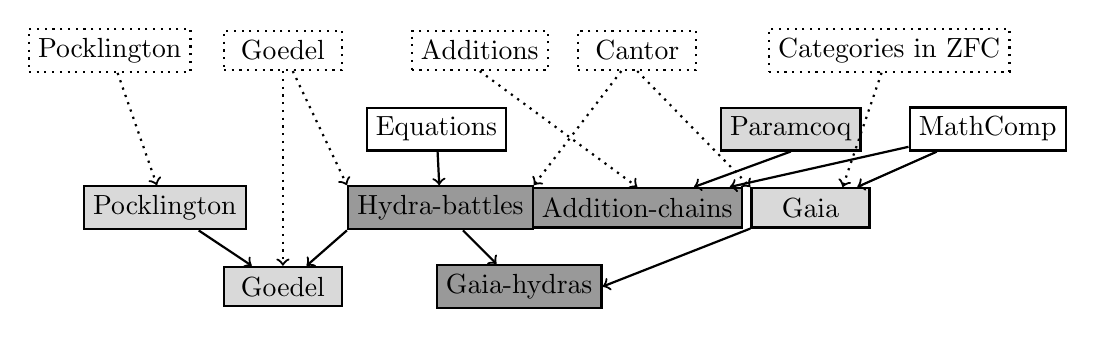
\begin{tikzpicture}[thick]

\begin{scope}[xshift=-6cm]
\node[rectangle, dotted,draw=black,minimum height=0.5cm,minimum width=1.5cm] (goedel) { Goedel };
\node[rectangle, dotted,draw=black,minimum height=0.5cm,minimum width=1.5cm,left of=goedel, node distance=2.2cm] (pock) { Pocklington };
\node[rectangle, dotted,draw=black,minimum height=0.5cm,minimum width=1.5cm,right of=goedel, node distance=2.5cm] (additions) { Additions };
\node[rectangle, dotted,draw=black,minimum height=0.5cm,minimum width=1.5cm,right of=additions, node distance=2cm] (cantor) { Cantor };

\node[rectangle, dotted,draw=black,minimum height=0.5cm,minimum width=1.5cm,right of=cantor, node distance=3.2cm] (cats) { Categories in ZFC };
\end{scope}

\begin{scope}[yshift=-1cm,xshift=0.45cm]
  \node[rectangle, draw=black,fill=gray!30,minimum height=0.5cm,minimum width=1.5cm] (paramcoq) { Paramcoq };
\node[rectangle, draw=black,minimum height=0.5cm,minimum width=1.5cm,right of=paramcoq, node distance=2.5cm] (mathcomp) { MathComp };
\node[rectangle, draw=black,minimum height=0.5cm,minimum width=1.5cm,node distance=2cm,left of=paramcoq, node distance=4.5cm] (equations) { Equations };
\end{scope}

\begin{scope}[yshift=-2cm,xshift=-4cm]
\node[rectangle, draw=black,fill=gray!80,minimum height=0.5cm,minimum width=1.5cm] (hydras) { Hydra-battles };
\node[rectangle, draw=black,fill=gray!30,minimum height=0.5cm,minimum width=1.5cm,left of=hydras, node distance=3.5cm] (pockcc) { Pocklington };
\node[rectangle, draw=black,fill=gray!80,minimum height=0.5cm,minimum width=1.5cm,right of=hydras, node distance=2.5cm] (chains) { Addition-chains };
\node[rectangle, draw=black,fill=gray!30,minimum height=0.5cm,minimum width=1.5cm,right of=chains, node distance=2.2cm] (gaia) { Gaia };
\end{scope}

\begin{scope}[yshift=-3cm,xshift=-6cm]
 \node[rectangle, draw=black,fill=gray!30,minimum height=0.5cm,minimum width=1.5cm] (goedelcc) { Goedel };
 \node[rectangle, draw=black,fill=gray!80,minimum height=0.5cm,minimum width=1.5cm,right of=goedelcc, node distance=3cm] (gaiahydras) { Gaia-hydras };
\end{scope}

\draw[->,dotted] (additions.south) -- (chains.north) ;
\draw[->,dotted] (goedel) -- (goedelcc) ;
\draw[->,dotted] (goedel) -- (hydras.north west) ;
\draw[->,dotted] (cantor) -- (hydras.north east) ;
\draw[->,dotted] (cantor.south) -- (gaia.north west) ;
\draw[->,dotted] (pock) -- (pockcc) ;
\draw[->,dotted] ([xshift=2.1cm]cats) -- (gaia) ;

\draw[->] (hydras) -- (gaiahydras) ;
\draw[->] (hydras.south west) -- (goedelcc) ;
\draw[->] (gaia.south west) -- (gaiahydras.east) ;

\draw[->] (equations) -- (hydras) ;
\draw[->] (mathcomp) -- (gaia) ;
\draw[->] (mathcomp) -- (chains) ;
\draw[->] (paramcoq.south) -- (chains) ;
\draw[->] (pockcc) -- (goedelcc) ;
\end{tikzpicture}
}
\caption{Genealogy and dependencies for \Hydras packages. Dotted boxes represent historical Coq contributions, while regular boxes represent maintained \coq packages. Dark gray packages are maintained in the \Hydras GitHub repository, while light gray packages are maintained in other \community repositories. Dotted lines represent \coq code ancestry, while regular lines represent direct code dependencies.}
  \label{fig:genealogy}
\end{figure}

Before the Ackermann sub-library was moved from the Goedel package repository to the \Hydras repository, the Goedel package had around 7,000 specification LOC and 38,000 proof LOC. Figure~\ref{fig:genealogy} and Table~\ref{tbl:loc} thus reveal that the seemingly large Coq formalization of G\"{o}del's incompleteness theorem can be viewed as a modestly-sized proof on top of general libraries for, on the one hand, first-order logic, primitive recursive functions, and Peano Arithmetic (Ackermann), and on the other hand, prime numbers and their properties (Pocklington).

\begin{table}[ht]
\centering
\footnotesize
\begin{tabular}{llllrr}
\hline
\textbf{Package name} & \textbf{Repository} & \textbf{Index identifier} & \textbf{Version} & \textbf{Spec LOC} & \textbf{Proof LOC}\\
\hline
Pocklington & \href{https://github.com/coq-community/pocklington}{\texttt{pocklington}} & \texttt{coq-pocklington} & \texttt{8.12.0} & 825 & 3,798 \\
Goedel & \href{https://github.com/coq-community/goedel}{\texttt{goedel}} & \texttt{coq-goedel} & \texttt{8.13.0} & 2,799 & 10,762 \\
Gaia & \href{https://github.com/coq-community/gaia}{\texttt{gaia}} & \texttt{coq-gaia} & \texttt{1.12} & 28,850 & 124,839 \\
Hydra-battles & \href{https://github.com/coq-community/hydra-battles}{\texttt{hydra-battles}} & \texttt{coq-hydra-battles} & \texttt{0.5} & 14,368 & 48,385 \\
Addition-chains & \href{https://github.com/coq-community/hydra-battles}{\texttt{hydra-battles}} & \texttt{coq-addition-chains} & \texttt{0.5} & 1,961 & 2,210 \\
Gaia-hydras & \href{https://github.com/coq-community/hydra-battles}{\texttt{hydra-battles}} & \texttt{coq-gaia-hydras} & \texttt{0.5} & 81 & 177 \\
\hline
\end{tabular}
\caption{Current numbers of lines of code for packages in the \Hydras galaxy.}
\label{tbl:loc}
\end{table}

In traditional software development, it is common for packages to continually depend on a large number of packages. In contrast, projects in the Coq ecosystem are often subject to ``dependency aversion'', where maintainers eschew depending on useful packages because it may lead to work in adapting to upstream changes. With \Hydras, we hope to demonstrate that projects with complex dependencies are feasible to manage using recent advances in build management and infrastructure.

% We could already talk a bit of the monorepo structure here, and
% defer some explanations on the tooling to the next section.

\section{Modernizing the build infrastructure}

\subsection{Documentation with \alectr}

The \Hydras book is written in LaTeX, but it makes very frequent references (about once per page, 274 snippets over 281 pages) to parts of the \coq development, showing definitions (Fig.~\ref{fig:Hprime}), computation results (Fig.~\ref{fig:Pow-evalPow17LetIn}), lemmas (Fig.~\ref{fig:Ex42E0}) and parts of  proof scripts (Fig.~\ref{fig:Ex42-schutte}). The order in which these references appear in the book is independent of the structure of our libraries, so we chose to maintain the book as a standalone document, separate from the \coq source code.  This contrasts with the \coqdoc approach, where explanatory prose is embedded within \coq source files (a detailed discussion of different approaches to documenting \coq developments can be found in \cite{alectryonpaper}).

Originally, we copied snippets from \coq sources into LaTeX manually, and recorded and inserted the corresponding outputs manually as well.  This approach is common, but brittle: changes to \coq definitions or lemmas had to be reflected in the book's sources, and we found multiple instances where the book and the \coq development had diverged.
 
We solved this maintenance issue by moving to \alectr, a tool that automatically records \coq proofs~\cite{alectryongithub}.  Instead of copy-pasting fragments into LaTeX, we now embed small LaTeX files automatically generated by \alectr from our \coq development.  Our build system guarantees that these LaTeX snippets are always up-to-date and consistent with the code (and, by comparing these snippets across releases of \coq or versions of \Hydras, we can easily spot unexpected changes).

Importing snippets into a LaTeX document was not one of the original use cases of Alectryon. Firstly, the original Alectryon did not have support for exporting to LaTeX. Secondly, it was geared towards documenting individual source files, where code and prose are interleaved within the same file. In this style, the code is documented in the same order as it is compiled.
We extended \alectr to support our needs by implementing a LaTeX backend, and by programming it to generate individual snippet files, one per \texttt{snippet} comment block.  The later part was straightforward: all it took was to build a custom \alectr \textit{driver}, a small (about 100 lines) Python program that leverages most of the \alectr toolchain but defines a custom frontend that understands our snippet annotations (and otherwise exposes the exact same command line as \alectr).

Once the infrastructure was in place, the transition happened gradually, over a few weeks: for each snippet of \coq code that was in the book, we had to take the following steps:

\begin{enumerate}
\item Mark the snippet in the \coq sources (we use special comments \texttt{(* begin snippet \textit{name} *)} … \texttt{(* end snippet \textit{name} *)})
\item Configure output display, using special \alectr annotations to configure what should be shown (only the inputs, inputs and outputs, some steps of the proof but not all, some proof states at key moments in a proof, etc.)
\item Replace the copy-pasted inputs and output in LaTeX with an \texttt{input} command.
\end{enumerate}

   \begin{figure}[h]
     \centering
     \fbox{
       \begin{minipage}[h]{1.0\linewidth}
         \inputsnippets{Pow_evalPow17LetIn}
       \end{minipage}}
  \caption{\label{fig:Pow-evalPow17LetIn}Automatically capturing the output of computations}
\end{figure}


  \begin{figure}[h]
    \centering
    \fbox{
      \begin{minipage}[h]{1.0\linewidth}
        \inputsnippets{E0_Ex42}
      \end{minipage}}
    \caption{A simple proof by computation}
    \label{fig:Ex42E0}
  \end{figure}



%\afterpage{\clearpage}

 


\begin{figure}[th]
  \centering
  
  

\fbox{\begin{minipage}[h]{1.0\linewidth}
  Let us prove again the equality $\omega+42+\omega^2= \omega^2$. We recall that $\omega^2$ is an abbreviation of $\phi_0(2)$,
\emph{i.e} the third  additive principal ordinal, and that \texttt{F} is a notation for the coercion which maps natural numbers to ordinals.

\inputsnippets{Schutte_Ex42a}


Our proof is very different from the computational proof of
Figure~\ref{fig:Ex42E0}.
By definition of additive principal ordinals, 
it suffices to prove the inequality $\omega+42< \phi_0(2)$.

\inputsnippets{Schutte_Ex42b}

Since the set \textit{AP} of additive principals  is closed under addition
(by Lemma \textit{AP\_plus\_closed}), it suffices to prove the inequalities $\omega<\omega^2$ and $42<\omega^2$.

\inputsnippets{Schutte_Ex42d, %to remove if short paper
  Schutte_Ex42c, Schutte_Ex42e}

\end{minipage}
}
\caption{A proof interleaved with text (from the book)}
  \label{fig:Ex42-schutte}
\end{figure}

\paragraph{Applications in other proof assistants.}
The Alectryon toolchain is intended to eventually support the languages of many proof assistants, and already has preliminary support for Lean~3. Our Alectryon extensions for snippet generation are in principle applicable to any language supported by Alectryon. However, snippet delimiters are language specific, and our tooling currently assumes Coq-compatible delimiters; we expect to lift this restriction in the near future. We view \Hydras as an incubator for experimental Alectryon features that, when deemed stable and useful, can be disseminated to a wider audience including users of other proof assistants.

\subsection{Technologies supporting the monorepo structure}

A monorepo (shorthand for monolithic repository) is a version control repository containing multiple independent or related packages.
%
Monorepos have gained increasing popularity following experiences in large companies such as Google, but are also used at a smaller scale for managing open source projects.
%
They are known to simplify the management of dependencies, making cross-packages changes, and refactorings~\cite{brito2018monorepos}.

%
One of the few early uses of monorepos in the Coq ecosystem was for the Mathematical Components library~\cite{MCB}, whose maintainers developed a custom build infrastructure to check multiple packages on each commit.
%
In light of that recent tooling improvements have made monorepo use easier, we chose to use an explicit monorepo structure for \Hydras in \community. Other \community projects have since adopted a similar structure.

In the context of \Hydras, we rely on the following tools.

\paragraph{The Dune build system~\cite{dune}.}
Dune was originally designed to build OCaml projects, but was recently extended to support Coq. Dune allows building packages contained in a single source tree separately, which is essential to be able to publish the different libraries contained in a single repository as separate (opam) packages to the Coq package index.

However, Dune is currently inconvenient for local IDE-based Coq code development and does not yet support building \coqdoc files.
%
Therefore, we still support building the whole project using \make via the \coqmakefile tool bundled with \coq, and we rely on this build system in our documentation generation pipeline.
%
We expect to migrate fully to Dune as soon as these limitations are lifted.

\paragraph{Docker-Coq-Action~\cite{martindorel2020dockercoq}.}
This GitHub Action provides a very simple way of setting up Continuous Integration (CI) for a Coq project with an opam file.
%
At the current time, we rely on it, together with the mathcomp Docker images~\cite{mathcompdocker}, to test our two main libraries, Hydra-battles and Addition-chains, with multiple versions of Coq.

\paragraph{The Coq Nix Toolbox~\cite{cohen:hal-03366644}.}
This toolbox, based on the Nix package manager, provides an alternative way of setting up CI for a Coq project (also relying on GitHub Actions).
%
We use this Nix-based CI for several things.

\begin{enumerate}
\item To test the build of the project (as a single unit) with \coqmakefile (whereas the Docker-based CI relies on the opam packages, which use Dune to build the libraries contained in the project).

\item To generate the documentation of the project (book in PDF format and \coqdoc HTML pages) by relying on the output of the \coqmakefile build.

\item To test the bridge to the Gaia library, because the Nix-based CI supports out-of-the-box caching of build dependencies.
%
Given that Gaia takes more than 5 minutes to build, this build is only done once, then reused at each new run of the CI.

\item To test compatibility with the Goedel library, which was made to depend on the Hydra-battles library since the Ackermann sub-library was moved from the former to the latter.
%
For this, we rely on the fact that the Coq Nix Toolbox has native support for generating a CI configuration that includes reverse dependency compatibility testing.
\end{enumerate}

The artifacts of the Nix builds are stored in the \community binary cache on Cachix~\cite{cachix}.
%
This means that a given version never has to be built twice and Continuous Integration can be almost instantaneous when no change has been made (e.g., after merging a pull request).

By relying on two different technologies for CI, we are able to fit a larger range of use cases, while also providing more assurance that the project does build correctly in a variety of configurations.
%
Given that the two technologies are well maintained (within \community), relying on both does not incur a significant cost, compared to the benefits they provide.

\section{Comparison of \Hydras with other Coq books}

We believe that Coq books can broadly be divided into two categories:
\begin{itemize}
\item \emph{Executable textbooks} that are in effect large, well-commented Coq programs from which other representations of the material (HTML, PDF) are derived using tools.
\item \emph{Traditional textbooks} generated from documentation languages such as LaTeX that are accompanied by standalone Coq formalizations and/or code snippets.
\end{itemize}
Table~\ref{tbl:books} shows a category breakdown for what we believe are the most prominent Coq books in English. Note that several traditional books, such as Coq'Art~\cite{BC04}, used custom tools during their writing process to keep code snippets synchronized with Coq. However, once a book is published, the accompanying code generally takes on a life of its own~\cite{CoqArtCommunity} and may come to substantially diverge from the book.

\begin{table}
  \centering
  \footnotesize
  \begin{tabular}{lll}
  \hline
  \textbf{Title} & \textbf{Year} & \textbf{Category}\\
  \hline
  Coq'Art~\cite{BC04} & 2004 & Traditional\\
  Software Foundations~\cite{SF} & 2007 & Executable\\
  Certified Programming with Dependent Types~\cite{chlipalacpdt2011} & 2011 &  Executable\\
  Program Logics for Certified Compilers~\cite{Appel2014} & 2014 & Traditional\\
  Programs and Proofs~\cite{Sergey:PnP} & 2014 & Executable\\
  Formal Reasoning About Programs~\cite{Chlipala2017} & 2017 & Traditional\\
  Computer Arithmetic and Formal Proofs~\cite{Boldo2017} & 2017 & Traditional\\
  Mathematical Components~\cite{MCB} & 2018 & Traditional\\
  \hline
  \end{tabular}
  \caption{Coq book categorization.}
  \label{tbl:books}
\end{table}

We believe the \Hydras electronic book has found an attractive set of tradeoffs between the properties of executable books and traditional books. Specifically, in an executable book, the proof assistant language places limits on the structure. For example, Coq may not permit repeating a definition from another file verbatim, since the definition uses variables that are not present in the current context. Thanks to our \alectr based toolchain, the \Hydras book can include ``live'' code fragments at any point in the text. And in contrast to traditional books, we validate the consistency of code fragments during every build of the electronic book. On the one hand, we follow executable books in providing ``continuous delivery'' of new revisions at a high pace. But on the other hand, we also aim to make regular timestamped versions compatible with specific versions of Coq, akin to new editions of traditional books.

Due to our reliance on LaTeX for writing the book, obtaining a book representation in HTML is more cumbersome than for executable books such as Software Foundations~\cite{SF} and Certified Programming with Dependent Types~\cite{chlipalacpdt2011}. Currently, we generate the Coq code documentation in HTML form separately from the book.

\section{Conclusion and perspectives}


\Hydras wants to provide a connection between scientific literature (\emph{e.g.},~\cite{KP82, KS81, schutte}) and proof assistant technology. For the mathematician, it can give a concrete view of the mathematical content, not only through full proofs, but also through illuminating computations: examples, functions associated with constructive proofs, etc. For the \coq learner, it provides a consistent set of examples,
allowing to present and compare various formalization and proving techniques. %It may be also used as a library, through opam packages.
It is also a medium sized library (more than 50,000 LOC), dependent on various tools and libraries of the \coq ecosystem, which may be also used to experiment with new maintenance techniques of the code and its documentation. To facilitate easy dissemination and reuse, all code and documentation is available under the permissive MIT license.





%\TODO{General Conclusion}



%\subsection{Perspectives}

%\subsection{Further extensions}

We plan to extend \Hydras in two main directions. Firstly, we plan to bridge the combinatorial results of \Hydras and the set-theoretic content of \gaia, enabling the transfer of many interesting theorems between the two packages. Secondly, we aim to write a formal proof in \coq of the original statement of Theorem~\ref{kp:thm2}, using O'Connor's formalization of Peano Arithmetic~\cite{Goedel}.
%
Moreover, \Hydras is not limited to the study of ordinal numbers and applications.
We are also developing a package about efficient exponentiation
algorithms, and aim to eventually include new topics. We invite new collaborators to join us in our efforts.

\section*{Acknowledgments}
\label{sect:acks}
We thank the anonymous reviewers for their comments, and we are grateful to the original authors and current maintainers of the Coq packages we use and depend on: José Grimm (Gaia), Russell O'Connor (Goedel), Matthieu Sozeau (Equations), the Mathematical Components team, Marc Lasson and Chantal Keller (Paramcoq), and the authors and maintainers of \coq and its associated tools.


\label{sect:bib}
\bibliographystyle{plain}
%\bibliographystyle{alpha}
%\bibliographystyle{unsrt}
%\bibliographystyle{abbrv}
% easychair.tex,v 3.5 2017/03/15

\documentclass{easychair}
%\documentclass[EPiC]{easychair}
%\documentclass[EPiCempty]{easychair}
%\documentclass[debug]{easychair}
%\documentclass[verbose]{easychair}
%\documentclass[notimes]{easychair}
%\documentclass[withtimes]{easychair}
%\documentclass[a4paper]{easychair}
%\documentclass[letterpaper]{easychair}

\usepackage{doc}
\usepackage{tikz}
\usepackage{tikzsymbols}
\usepackage{pifont}
\newtheorem{theorem}{Theorem}
\usetikzlibrary{arrows}

%\usepackage[firstpageonly=false, color={[gray]{0.5}},
%   scale=2.0, text=DRAFT]{draftwatermark}
% -------------------------------
%%%% For Alectryon

\usepackage{texments}
%%% for movies by alectryon
\usepackage{alectryon}
\usepackage{pygments}
%%% One hypothesis per line 
\makeatletter
\renewcommand{\alectryon@hyps@sep}{\alectryon@nl}
\makeatother

%%% \snippets{A,B,C,…} inputs a series of snippets as one block (with \itemsep
%%% between them).  A, B, C should be paths to files in snippets/.
\usepackage{etoolbox}
\makeatletter
\newcommand{\inputsnippets}[1]
  {{\setlength{\itemsep}{1pt}\setlength{\parsep}{0pt}% Adjust spacing
    \alectryon@copymacros\begin{io}
      \forcsvlist{\item\@inputsnippet}{#1}
    \end{io}}}
\let\input@old\input % Save definition of \input
\newcommand{\@inputsnippet}[1]
  {{\renewenvironment{alectryon}{}{}% Skip \begin{alectryon} included in snippet
    \input@old{#1}}}
\makeatother

%---------------------------- 
\newcommand{\canonseq}[2]{\mbox{$\{#1\}(#2)$}}

\usepackage{varioref}
\newtheorem{todo}{To do}
\usepackage{amsfonts, afterpage}
\usepackage{xspace}

\newcommand{\easychair}{\textsf{easychair}}
\newcommand{\miktex}{MiK{\TeX}}
\newcommand{\texniccenter}{{\TeX}nicCenter}
\newcommand{\makefile}{\texttt{Makefile}}
\newcommand{\latexeditor}{LEd}

%\makeindex

%% Front Matter
%%
% Regular title as in the article class.
%
% \title{Hydras,  Ordinals \& Co.   \\
%   A library in Coq of entertaining formal mathematics}

\title{Hydras \& Co.: Formalized mathematics in Coq\\
 for inspiration and entertainment
}

\author{
Pierre Castéran \inst{1}
\and
    Jérémy Damour \inst{2}
\and
Karl Palmskog \inst{3}
\and Clément Pit-Claudel \inst{4}
\and Théo Zimmermann \inst{5}
}


\institute{
Univ. Bordeaux, CNRS, Bordeaux INP, LaBRI, UMR 5800, F-33400 Talence, France  %\\
 % \email{pierre.casteran@labri.fr}
\and
Univ. de Paris, F-75013 Paris, France
\and
KTH Royal Institute of Technology, Stockholm, Sweden
\and
MIT CSAIL, Cambridge, Massachusetts, USA
\and
Inria, Univ. de Paris, CNRS, IRIF, UMR 8243, F-75013 Paris, France
}



\authorrunning{Castéran, Damour, Palmskog, Pit-Claudel and Zimmermann}

\titlerunning{\Hydras}

\newcommand{\TODO}[2][]{[\textcolor{red}{TODO (#1):} \emph{#2}]}
\newcommand{\coq}{Coq\xspace}
\newcommand{\coqdoc}{Coqdoc\xspace}
\newcommand{\coqmakefile}{\texttt{coq\_makefile}\xspace}
\newcommand{\community}{Coq-community\xspace}
\newcommand{\gaia}{Gaia\xspace}
\newcommand{\alectr}{Alectryon\xspace}
\newcommand{\equations}{Equations\xspace}
\newcommand{\Hydras}{Hydras \& Co$\text.$\xspace}
\newcommand{\make}{\texttt{make}\xspace}
%\newcommand{\Hydras}{Hydra-battles\xspace}

\begin{document}

\maketitle


\begin{abstract}
  \Hydras is a collaborative library of discrete mathematics for the
  \coq proof assistant, developed as part of the \community organization
  on GitHub. The Coq code is accompanied
  by an electronic book, generated with the help of the \alectr
  literate proving tool. We present the evolution of the mathematical
  contents of the library since former presentations at JFLA meetings.
  Then, we describe how the structure of the project is determined
  by two requirements which must be continuously satisfied.
  First, the Coq code needs to be compatible with its ever-evolving
  dependencies (the Coq proof assistant and several Coq packages both from
  inside and outside \community) and reverse dependencies (\community
  projects that depend on it). Second, the book needs to be consistent
  with the Coq code, which undergoes frequent changes to improve
  structure and include new material. We believe \Hydras demonstrates
  that books on formalized mathematics are not limited to
  providing exposition of theories and reasoning techniques---they
  can also provide inspiration and entertainment that transcend educational goals.
\end{abstract}


% \setcounter{tocdepth}{2}
% {\small
% \tableofcontents}


%------------------------------------------------------------------------------
\section{Introduction}
\label{sect:introduction}

\subsection{Background}

Libraries of formalized mathematics based on proof assistants, such as \coq, Lean, and Isabelle/HOL, are continually growing in size and scope.
For example, Mathlib for Lean and the core set of projects in the Mathematical Components family for Coq both amount to hundreds of thousands of lines of code (LOC) and tens of thousands of definitions and theorems~\cite{Nie2020a, Mathlib}. However, after a key mathematical definition or result is added to a library, it must be \emph{documented and maintained}~\cite{vanDoorn2020,alectryonpaper}.

Maintenance includes not only adaptation to changes in new proof assistant versions, but also reorganization to accommodate new contributions. Documentation is usually two-fold: \emph{source code comments} that describe specific definitions and results in-line and \emph{books} that carefully introduce the library and its idioms~\cite{MCB,TheoremProvingLean4}. The former tends to be terse and dense and serves experienced users, while the latter is more long-winded and exhaustive and serves beginners. As a library changes and expands, all its documentation needs to be made consistent and complete. Authors use many techniques, including literate programming~\cite{Knuth1984} and custom tools, to pretty-print and check source code snippets and generate proof assistant output.

While books that document proof assistant libraries are valuable to beginners, the purpose of recently published books is mainly instrumental, i.e., to teach a certain topic or technique. We believe that books and libraries can instead become \emph{ends in themselves}---not just sources of exposition and learning, but also sources of inspiration and entertainment.

\subsection{Vision}
The \Hydras project, part of \community on GitHub~\cite{CoqCommunity}, aims to be an experimental platform for the collaborative development of documented libraries of formal proofs. \community is a community organization that the first and last authors founded in 2018 with two goals in mind: providing a solution for the long-term maintenance of interesting open source \coq packages, and working collaboratively on documentation projects. The \Hydras project demonstrates that these two goals are not independent: interesting \coq packages can become the basis for new documentation.
%
This umbrella project now includes evolved versions of the former Cantor and Additions libraries~\cite{CantorContrib,AdditionsContrib} (under the new names of Hydra-battles and Addition-chains), the Ackermann sub-library extracted from Russel O'Connor's Goedel library~\cite{OConnor05, Goedel}, and a bridge to the \gaia library by José Grimm~\cite{Gaia,grimm:hal-00911710}.
%
By following this approach of commenting interesting \coq packages, we provide new documentation content that contributes to the diversity of the thriving \coq ecosystem.

We call on the \coq users in the JFLA community and beyond to come and join us in this effort, by bringing new interesting projects which are worth presenting to \coq learners, \emph{a.k.a.} \coq users, and guiding them in their exploration.
%
We also always have project ideas to extend further our explorations and anyone is welcome to join the team by sending small or larger contributions through pull requests.
%
The current state of the project is already the result of such evolutions after several of us contributed project solutions and new proposals to the initial version of the first author.

Futhermore, contrary to traditionally published books, the ``book'' that forms part of this project is intended to be forever evolving. As new \coq formalization patterns and proof techniques appear, the book can be adapted to demonstrate their use (in case they fit well with our applications).
%
By using modern maintenance techniques such as continuous integration and deployment, we can ensure that this documentation stays up to date with the latest \coq releases. With \alectr~\cite{alectryonpaper, alectryongithub}, we ensure that code and documentation are always in sync.

\subsection{Hydra games}

We chose to build our library and book on two simple themes which allow many variations: computing powers in a monoid, and Kirby and Paris' hydra battles. In the interest of space, we will only present the second theme in this paper.


Hydra games (also known as \emph{Hydra battles}) appear in an article published in 1982 by two mathematicians, 
Laurie Kirby and Jeff Paris: \emph{Accessible Independence Results for Peano Arithmetic}~\cite{KP82}.
This article describes a game between two players: Hercules and a hydra.
A short description of the game  can be found in~\cite{bauer2008, KP82, JFLA2018paper}. One can also play with
Andrej Bauer's simulator~\cite{BauerHydra}.
In a few words:
\begin{itemize}
\item A hydra is a finite tree, traditionally presented with the root at the bottom, the leaves of which are called \emph{heads}
  (Figure~\ref{fig:round}).
\item At every round, Hercules chops off one head of the hydra. If the head is at a distance greater than 1 from the root,
  then some sub-tree $h$ of the hydra is copied a certain amount $n$ of times. The number $n$ of copies and the sub-tree $h$ may depend on the considered variant of the game
  and the time elapsed since the beginning of the fight.
  Figure~\ref{fig:round} shows an example with $n=2$.
\end{itemize}



\begin{figure}[h]
  \centering
  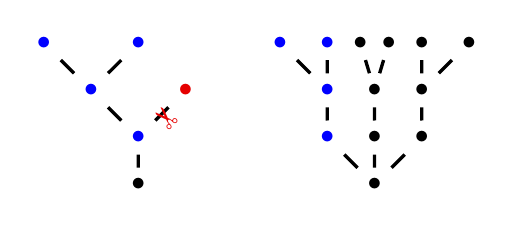
\begin{tikzpicture}[very thick, scale=0.3]
  \node (h1) at (4,0){$\bullet$};
  \node[blue] (h2) at (4,2){$\bullet$};
  \node[blue] (h3) at (2,4){$\bullet$};
  \node[blue] (h4) at (0,6){$\bullet$};
  \node[blue] (h5) at (4,6){$\bullet$};
  \node[red!90!black] (h6) at (6,4){$\bullet$};
  \draw (h1) -- (h2) ;
  \draw (h2) -- (h3) ;
  \draw (h2) -- node[red!90!black,font=\small,sloped,shift={(0.01,-0.075)},rotate=90]{\textbf{\ding{34}}} (h6);
  \draw (h3) -- (h4) ;
  \draw (h3) -- (h5) ;
 
\node (hn1) at (14,0){$\bullet$};
\node[blue] (hn2) at (12,2) {$\bullet$};
\node[blue] (hn3) at (12,4) {$\bullet$};
\node[blue] (hn4) at (10,6){$\bullet$};
  \node[blue] (hn5) at (12,6){$\bullet$};
  \draw (hn1) -- (hn2) ;
  \draw (hn2) -- (hn3) ;
  \draw (hn3) -- (hn4) ;
  \draw (hn3) -- (hn5) ;
\node (hn2b) at (14,2) {$\bullet$};
\node (hn3b) at (14,4) {$\bullet$};
\node (hn4b) at (13.4,6){$\bullet$};
  \node (hn5b) at (14.6,6){$\bullet$};
  \draw (hn1) -- (hn2b) ;
  \draw (hn2b) -- (hn3b) ;
  \draw (hn3b) -- (hn4b) ;
  \draw (hn3b) -- (hn5b) ;
  \node (hn2c) at (16,2) {$\bullet$};
\node (hn3c) at (16,4) {$\bullet$};
\node (hn4c) at (16,6){$\bullet$};
  \node (hn5c) at (18,6){$\bullet$};
  \draw (hn1) -- (hn2c) ;
  \draw (hn2c) -- (hn3c) ;
  \draw (hn3c) -- (hn4c) ;
  \draw (hn3c) -- (hn5c) ;
\end{tikzpicture}

  \caption{Two successive states of a hydra in a battle.  Hercules chopped off the rightmost head of the hydra (red), and the whole left tree except the root node (blue) was copied twice.}
  \label{fig:round}
\end{figure}



 %  \begin{figure}[htb]
% \centering
% \begin{tikzpicture}[very thick, scale=0.3]
% \node (foot) at (10,0) {$\bullet$};
% \node (N1) at (2,2) {$\bullet$};
% \node (N2) at (10,2) {$\bullet$};
% \node (N22) at (7,2) {$\bullet$};
% \node (N3) at (14,2) {$\bullet$};
% \node (N4) at (18,2) {$\Smiley[2][green]$};
% \node (N5) at (0,4) {$\bullet$};
% \node (N6) at (2,5) {$\Smiley[2][green]$};
% \node (N7) at (4,6) {$\Smiley[2][green]$};
% \node (N88) at (7,4) {$\bullet$};
% \node (N8) at (10,4) {$\bullet$};
% \node (N9) at (14,6) {$\Smiley[2][green]$};
% \node (N10) at (0,8) {$\Smiley[2][green]$};
% \node (N11) at (10,7) {$\Smiley[2][green]$};
% \node (N111) at (7,7) {$\Smiley[2][green]$};
% \draw (foot) to [bend left=10] (N1);
% \draw (foot) -- (N2);
% \draw (foot) -- (N22);
% \draw (foot) -- (N3);
% \draw (foot) -- (N4);
% \draw (N1) to  (N5);
% \draw (N1) to   [bend left=10] (N6);
% \draw (N1) to   [bend right=20] (N7);
% \draw (N2) to  (N8);
% \draw (N22) to  (N88);
% \draw (N8) to  (N11);
% \draw (N88) to  (N111);
% \draw (N3) to  (N9);
% \draw (N5) to  (N10);
% \end{tikzpicture}
% \caption{The hydra associated with the ordinal $\omega^{\omega+2}+\omega^\omega \times 2 + \omega + 1$ \label{fig:iota-example}}

% \end{figure}

Kirby and Paris proved the following theorems, applying
combinatorial results about ordinal numbers by Jussi Ketonen and Robert Solovay~\cite{KS81}.

\begin{theorem}
  In the Hydra game, Hercules eventually wins, whichever the strategy of both players:
  choice of a head to chop off, choice of the number of copies.
 \label{kp:thm1}
\end{theorem}

\begin{theorem}
  Theorem~\ref{kp:thm1} cannot be proved in Peano Arithmetic. \label{kp:thm2}
\end{theorem}

The contrast between the simplicity of the statements above and the complexity of their proofs convinced us that it is a good theme for a commented library~\cite{HydraBattles} of formal proofs written for the \coq proof assistant~\cite{Coq}. 

Complex formalizations and proofs are explained in the book.
% an  electronic book~\cite{HydraBook} (PDF document of over 280 pages).
Whenever various reasonable choices exist, we try to present and compare the alternatives.
  For instance, Figures~\ref{fig:Ex42E0} and \ref{fig:Ex42-schutte} show two radically different proofs of the equality
  $\omega+42+\omega^2=\omega^2$. The first one is a simple proof by computation, the second one shows how this equality
  is a consequence of the axioms of the set-theoretic model  by Kurt Schütte~\cite{schutte}. 

This work is also an opportunity to 
 provide concrete examples of formalization and proof techniques: operational type classes, functions defined by  equations, dependently typed functions, etc. It may be also used as a library on ordinal numbers, for instance for proving termination properties.
%
 Prior stages of this project have already been presented at
 JFLA~\cite{PCiota, JFLA2018paper}.
In this paper, we present recent evolutions of the library: new results, interaction with the \community project~\cite{CoqCommunity}, and documentation generated with \alectr~\cite{alectryonpaper, alectryongithub}.

\section{Recent developments}
The 2018 article~\cite{JFLA2018paper} presented a formal proof of the following theorem:

\begin{theorem}
  Let $\mu$ be any ordinal strictly less than $\epsilon_0$.
  There is no function mapping hydras to the segment $[0,\mu)$ that could be used as a measure in proving termination for \emph{any} hydra battle.\label{thm3}
\end{theorem}

Our proof was based on the construction of a battle between Hercules and the hydra where the
number of copies at each round was given by the elimination of an existential quantifier. So, it was mandatory to consider the class of \emph{all} hydra battles, or, equivalently, the class of battles where the hydra choses arbitrarily its number $n$ of copies at every round of the battle.

Unfortunately, the examples  most commonly shown in the literature
(see for instance~\cite{KP82, bauer2008, BauerHydra}) 
assume that the hydra grows $k$ copies at step $k$ of the game, which is incompatible with our proof.
We prove now that Theorem~\ref{thm3} still holds with these typical battles.
%by borrowing new combinatorial results from~\cite{KS81}.
Since we are looking  for a minoration of the length of such battles,
we can work with the following hypotheses and invariants, 
without any loss of generality.
 
 \begin{itemize}
   \item The game starts at an initial step $k=i$, where $i$ is any natural number.
   \item Hercules always chops off the rightmost head of the hydra.
   \item  The hydra is always the tree representation of some ordinal strictly below $\epsilon_0$ in Cantor normal
     form (thus, the rightmost branch is also one of the shortest).
     For instance, Figure~\ref{fig:round} shows the hydras respectively associated with  $\omega^{\omega^2+1}$ and $\omega^{\omega^2}\times 3$.
 \end{itemize}
 
 In mathematical terms, if at step $k\geq i$, the hydra is associated with the ordinal $\alpha$, at step $k+1$ it is associated with
 $\canonseq{\alpha}{k+1}$, \emph{i.e.} the $(k+1)$th element of the canonical sequence of $\alpha$~\cite{KS81}. In the following,  the expression ``the hydra $\alpha$'' is an abbreviation of ``the hydra associated with the ordinal $\alpha$''.
 
 Our new proof of Theorem~\ref{thm3} is based on a systematic study of strictly decreasing sequences of ordinals below $\epsilon_0$, borrowed from Ketonen and Solovay~\cite{KS81}, and the formalization of which is described in detail  in chapters 5 and 6 of~\cite{HydraBook}.

 Besides  Theorem~\ref{thm3}, we study also the number of steps of a battle:
Let $\alpha<\epsilon_0$ be an ordinal. 
We prove that  the number of steps of the battle starting with
$\alpha$ at step $i$ is greater or equal than
$H'_\alpha(i)-i$, where $H'$ is a slight variant of the Hardy hierarchy of rapidly growing functions~\cite{BW85, KS81, Promel2013, Wainer1970}.  The function $H'_\alpha$ is defined by transfinite recursion over $\alpha$ on Figures~\ref{fig:hardy-math}
and~\ref{fig:Hprime}.


\begin{figure}[h]
\begin{align}
  H'_0(i) & = i\\
  H'_\alpha(i) &= H'_{(\canonseq{\alpha}{i+1})}(i)  \quad\textit{if $\alpha$ is a limit ordinal}\\
  H'_{\alpha}(i) &=H'_\beta(i+1) \quad\textit{if $\alpha=\beta+1$}
\end{align}  
  \caption{The $H'$ rapidly growing hierarchy of arithmetical functions}
  \label{fig:hardy-math}
\end{figure}


\begin{figure}[h]
  \centering
  \fbox{
    \begin{minipage}[h]{1.0\linewidth}
 \inputsnippets{Hprime_HprimeDef}     
    \end{minipage}}
 \caption{$H'$ definition with the \texttt{coq-equations}
 plug-in~\cite{sozeau:hal-01671777}}
\label{fig:Hprime}
\end{figure}


Using $H'$s equations as rewrite rules, we can study a concrete example. We take the hydra of figure~\ref{fig:start} and $i=0$ as initial configuration. 
By a sequence of rewritings and inductions, we prove that the number of steps of the considered battle is greater or equal than $2^{2^N}$, where $N=2^{70}-1$.
By comparison with the diagonalized Ackermann function $\lambda\,i.\,A(i,i)$, we prove also that, for $\alpha\geq\omega^\omega$, 
the function computing the length of the battle starting with the hydra $\alpha$ and the initial step $i$ is not primitive recursive.

\begin{figure}[h]
  \centering
  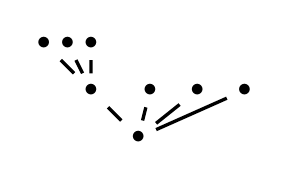
\begin{tikzpicture}[very thick, scale=0.3]
  \node (h1) at (4,0){$\bullet$};
  \node (h2) at (2,2){$\bullet$};
  \node (h3) at (0,4){$\bullet$};
  \node (h4) at (1,4){$\bullet$};
  \node (h5) at (2,4){$\bullet$};
  \node (h6) at (4.5,2){$\bullet$};
  \node (h7) at (6.5,2){$\bullet$};
  \node (h8) at (8.5,2){$\bullet$};
    \draw (h1) -- (h2) ;
    \draw (h2) -- (h3) ;
    \draw (h2) -- (h4) ;
    \draw (h2) -- (h5) ;
    \draw (h1) -- (h6) ;
    \draw (h1) -- (h7) ;
    \draw (h1) -- (h8);
 \end{tikzpicture}

  \caption{The hydra associated with the ordinal $\omega^3+3$}
  \label{fig:start}
\end{figure}




\label{sect:not-pr}

%\TODO[Clément]{Could we use a font with ligatures?}


\section{Integration with \community}

\subsection{Background}

\community is an informal organization run by volunteer Coq users on GitHub that aims to maintain interesting open source Coq projects for the long term and facilitate collaboration among Coq users on documentation, tooling, etc. \community was created in 2018, inspired by the {Elm Community} organization~\cite{zimmermann:tel-02451322}.
%
Such ``Community Package Maintenance Organizations'' exist in many software ecosystems, as they avoid the common problem of an important package becoming unmaintained after its author has moved on to other projects or has disappeared~\cite{zimmermann2021grounded}.

In the case of \coq, this problem is likely even more prevalent than in other ecosystems, as many packages are created by graduate students or researchers for a specific paper and not planned to be maintained for the long term by authors.
%
However, authors are generally open to having someone else who expresses interest in their work take over package maintenance.
%

\community makes it easy to change maintainers by defining a process for transferring or forking an unmaintained package, tooling for setting up good maintenance practices (such as continuous integration), and by making it possible for someone to take over a package without making a long-term commitment (as maintainers who drop out can easily be replaced by some other volunteers).

As of 2021, \community hosts over 50 projects maintained by over 30 volunteers.
%
The hosted projects come from a variety of origins.
%
Some had been maintained in the past by the \coq development team on behalf of the authors, but this meant that only minimal changes required to make the project build with new \coq versions were performed.
%
Some were still maintained by their original authors, but were transferred to enable other users to help out with maintenance and facilitate adoption of best practices on, e.g., continuous integration.
%
Others were simply unmaintained and were revived after their transfer to \community.

Given the objectives of \community, we believe it makes sense to propose a transfer anytime we encounter an interesting Coq project that is insufficiently maintained.
%
After a transfer, the \community maintainers are explicitly allowed to perform large changes and refactorings.
%
This means, for instance, that we can consolidate packages by merging them, or split up a single package into several packages.

\subsection{Integration of primitive recursive functions}

In order to prove formally that the length of the
kind of hydra battles we consider is not given by any primitive recursive function, we chose to use a formalization of primitive recursive functions that was originally part of Russell O'Connor's formal proof of G\"{o}del's first incompleteness theorem~\cite{OConnor05, Goedel}.
For this purpose, and above all in consideration of the scientific interest of this contribution, we decided to host and maintain O'Connor's work in \community.

Since computability is a key topic in computer science teaching and O'Connor's library is a nice illustration of dependently typed programming, we decided to devote a full chapter (chapter 9 of~\cite{HydraBook}) to the formalization of primitive recursive functions, with comments on the definitions and proofs and (counter-)examples and exercises. As part of the writing process, we made the formalization into a new sub-library of the Hydra-battles library, dubbed Ackermann.

\subsection{Towards a bridge to \gaia}

The \gaia project by Jos\'e Grimm aimed to formalize mathematics in \coq in the style of Nicolas Bourbaki. The formalization of the first book in the Elements of Mathematics series by Bourbaki, on the theory of sets, was initially described in a technical report in July 2009~\cite{Grimm2009a}. The set-theoretic axioms and basic definitions in \gaia were derived from an earlier development by Carlos Simpson~\cite{Simpson2004,CatsZFCContrib}. Grimm then wrote (and continually updated) technical reports describing the formalization of Bourbaki's two subsequent books~\cite{Grimm2009b,Grimm2016} and additional topics in number theory~\cite{grimm:hal-00911710,Grimm2014}, before he passed away in 2019.

In 2020, members of \community transferred the \gaia source code to GitHub and adapted it for recent releases of the Mathematical Components library, which \gaia heavily relies on. Anonymous volunteers (``collaborators of Nicolas Bourbaki'') then finished the only in-progress proof left by Grimm. At around 155,000 LOC, \gaia is currently one of the largest maintained open source \coq projects~\cite{Gaia}.

\gaia contains definitions of ordinals in Cantor and Veblen normal form~\cite{grimm:hal-00911710}, adapted from the historical Cantor contribution~\cite{CantorContrib}. The data types for ordinals are essentially defined the same way as in \Hydras, but they are not identical inside \coq, e.g., due to residing in different modules. There are also minor differences in how ordinal arithmetic is implemented, due to the different evolutionary paths taken since divergence from the ancestor library.

As an initial step in bridging \gaia and \Hydras, we were able to establish a correspondence between both implementations of ordinals through rewriting lemmas. For instance, we proved that multiplication of ordinals in Cantor normal form in \Hydras refine \gaia's corresponding multiplication operation, and then imported \gaia's proof of associativity of the multiplication almost for free.

The initial draft bridge code mostly uses the SSReflect proof language and idioms from the Mathematical Components library. We made this design decision since we believe it is less challenging to reason about Hydra-battles code using SSReflect and MathComp than to reason about Gaia without SSReflect.

\subsection{Package Genealogy, Dependencies, and Organization}

Both due to its prior stages~\cite{PCiota,JFLA2018paper} and the recent integrations described just above, the current \Hydras \coq code has a complex inheritance. Figure~\ref{fig:genealogy} illustrates the relationships between \Hydras packages and show their ancestry from historical Coq contributions. To indicate the scope and relative sizes of packages, Table~\ref{tbl:loc} breaks down lines of code for each package in the \Hydras galaxy, as reported by the \texttt{coqwc} tool, and lists their repository names in \community and identifiers in the \coq opam package index~\cite{CoqPackageIndex}.

\begin{figure}[ht]
\centering
{\footnotesize
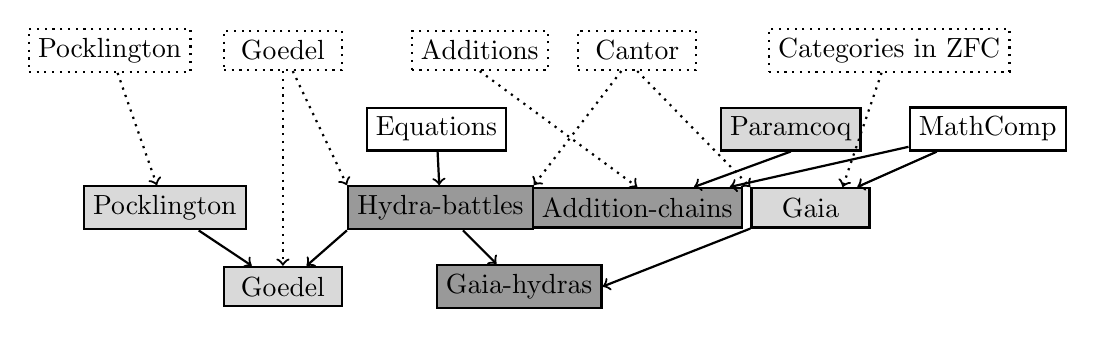
\begin{tikzpicture}[thick]

\begin{scope}[xshift=-6cm]
\node[rectangle, dotted,draw=black,minimum height=0.5cm,minimum width=1.5cm] (goedel) { Goedel };
\node[rectangle, dotted,draw=black,minimum height=0.5cm,minimum width=1.5cm,left of=goedel, node distance=2.2cm] (pock) { Pocklington };
\node[rectangle, dotted,draw=black,minimum height=0.5cm,minimum width=1.5cm,right of=goedel, node distance=2.5cm] (additions) { Additions };
\node[rectangle, dotted,draw=black,minimum height=0.5cm,minimum width=1.5cm,right of=additions, node distance=2cm] (cantor) { Cantor };

\node[rectangle, dotted,draw=black,minimum height=0.5cm,minimum width=1.5cm,right of=cantor, node distance=3.2cm] (cats) { Categories in ZFC };
\end{scope}

\begin{scope}[yshift=-1cm,xshift=0.45cm]
  \node[rectangle, draw=black,fill=gray!30,minimum height=0.5cm,minimum width=1.5cm] (paramcoq) { Paramcoq };
\node[rectangle, draw=black,minimum height=0.5cm,minimum width=1.5cm,right of=paramcoq, node distance=2.5cm] (mathcomp) { MathComp };
\node[rectangle, draw=black,minimum height=0.5cm,minimum width=1.5cm,node distance=2cm,left of=paramcoq, node distance=4.5cm] (equations) { Equations };
\end{scope}

\begin{scope}[yshift=-2cm,xshift=-4cm]
\node[rectangle, draw=black,fill=gray!80,minimum height=0.5cm,minimum width=1.5cm] (hydras) { Hydra-battles };
\node[rectangle, draw=black,fill=gray!30,minimum height=0.5cm,minimum width=1.5cm,left of=hydras, node distance=3.5cm] (pockcc) { Pocklington };
\node[rectangle, draw=black,fill=gray!80,minimum height=0.5cm,minimum width=1.5cm,right of=hydras, node distance=2.5cm] (chains) { Addition-chains };
\node[rectangle, draw=black,fill=gray!30,minimum height=0.5cm,minimum width=1.5cm,right of=chains, node distance=2.2cm] (gaia) { Gaia };
\end{scope}

\begin{scope}[yshift=-3cm,xshift=-6cm]
 \node[rectangle, draw=black,fill=gray!30,minimum height=0.5cm,minimum width=1.5cm] (goedelcc) { Goedel };
 \node[rectangle, draw=black,fill=gray!80,minimum height=0.5cm,minimum width=1.5cm,right of=goedelcc, node distance=3cm] (gaiahydras) { Gaia-hydras };
\end{scope}

\draw[->,dotted] (additions.south) -- (chains.north) ;
\draw[->,dotted] (goedel) -- (goedelcc) ;
\draw[->,dotted] (goedel) -- (hydras.north west) ;
\draw[->,dotted] (cantor) -- (hydras.north east) ;
\draw[->,dotted] (cantor.south) -- (gaia.north west) ;
\draw[->,dotted] (pock) -- (pockcc) ;
\draw[->,dotted] ([xshift=2.1cm]cats) -- (gaia) ;

\draw[->] (hydras) -- (gaiahydras) ;
\draw[->] (hydras.south west) -- (goedelcc) ;
\draw[->] (gaia.south west) -- (gaiahydras.east) ;

\draw[->] (equations) -- (hydras) ;
\draw[->] (mathcomp) -- (gaia) ;
\draw[->] (mathcomp) -- (chains) ;
\draw[->] (paramcoq.south) -- (chains) ;
\draw[->] (pockcc) -- (goedelcc) ;
\end{tikzpicture}
}
\caption{Genealogy and dependencies for \Hydras packages. Dotted boxes represent historical Coq contributions, while regular boxes represent maintained \coq packages. Dark gray packages are maintained in the \Hydras GitHub repository, while light gray packages are maintained in other \community repositories. Dotted lines represent \coq code ancestry, while regular lines represent direct code dependencies.}
  \label{fig:genealogy}
\end{figure}

Before the Ackermann sub-library was moved from the Goedel package repository to the \Hydras repository, the Goedel package had around 7,000 specification LOC and 38,000 proof LOC. Figure~\ref{fig:genealogy} and Table~\ref{tbl:loc} thus reveal that the seemingly large Coq formalization of G\"{o}del's incompleteness theorem can be viewed as a modestly-sized proof on top of general libraries for, on the one hand, first-order logic, primitive recursive functions, and Peano Arithmetic (Ackermann), and on the other hand, prime numbers and their properties (Pocklington).

\begin{table}[ht]
\centering
\footnotesize
\begin{tabular}{llllrr}
\hline
\textbf{Package name} & \textbf{Repository} & \textbf{Index identifier} & \textbf{Version} & \textbf{Spec LOC} & \textbf{Proof LOC}\\
\hline
Pocklington & \href{https://github.com/coq-community/pocklington}{\texttt{pocklington}} & \texttt{coq-pocklington} & \texttt{8.12.0} & 825 & 3,798 \\
Goedel & \href{https://github.com/coq-community/goedel}{\texttt{goedel}} & \texttt{coq-goedel} & \texttt{8.13.0} & 2,799 & 10,762 \\
Gaia & \href{https://github.com/coq-community/gaia}{\texttt{gaia}} & \texttt{coq-gaia} & \texttt{1.12} & 28,850 & 124,839 \\
Hydra-battles & \href{https://github.com/coq-community/hydra-battles}{\texttt{hydra-battles}} & \texttt{coq-hydra-battles} & \texttt{0.5} & 14,368 & 48,385 \\
Addition-chains & \href{https://github.com/coq-community/hydra-battles}{\texttt{hydra-battles}} & \texttt{coq-addition-chains} & \texttt{0.5} & 1,961 & 2,210 \\
Gaia-hydras & \href{https://github.com/coq-community/hydra-battles}{\texttt{hydra-battles}} & \texttt{coq-gaia-hydras} & \texttt{0.5} & 81 & 177 \\
\hline
\end{tabular}
\caption{Current numbers of lines of code for packages in the \Hydras galaxy.}
\label{tbl:loc}
\end{table}

In traditional software development, it is common for packages to continually depend on a large number of packages. In contrast, projects in the Coq ecosystem are often subject to ``dependency aversion'', where maintainers eschew depending on useful packages because it may lead to work in adapting to upstream changes. With \Hydras, we hope to demonstrate that projects with complex dependencies are feasible to manage using recent advances in build management and infrastructure.

% We could already talk a bit of the monorepo structure here, and
% defer some explanations on the tooling to the next section.

\section{Modernizing the build infrastructure}

\subsection{Documentation with \alectr}

The \Hydras book is written in LaTeX, but it makes very frequent references (about once per page, 274 snippets over 281 pages) to parts of the \coq development, showing definitions (Fig.~\ref{fig:Hprime}), computation results (Fig.~\ref{fig:Pow-evalPow17LetIn}), lemmas (Fig.~\ref{fig:Ex42E0}) and parts of  proof scripts (Fig.~\ref{fig:Ex42-schutte}). The order in which these references appear in the book is independent of the structure of our libraries, so we chose to maintain the book as a standalone document, separate from the \coq source code.  This contrasts with the \coqdoc approach, where explanatory prose is embedded within \coq source files (a detailed discussion of different approaches to documenting \coq developments can be found in \cite{alectryonpaper}).

Originally, we copied snippets from \coq sources into LaTeX manually, and recorded and inserted the corresponding outputs manually as well.  This approach is common, but brittle: changes to \coq definitions or lemmas had to be reflected in the book's sources, and we found multiple instances where the book and the \coq development had diverged.
 
We solved this maintenance issue by moving to \alectr, a tool that automatically records \coq proofs~\cite{alectryongithub}.  Instead of copy-pasting fragments into LaTeX, we now embed small LaTeX files automatically generated by \alectr from our \coq development.  Our build system guarantees that these LaTeX snippets are always up-to-date and consistent with the code (and, by comparing these snippets across releases of \coq or versions of \Hydras, we can easily spot unexpected changes).

Importing snippets into a LaTeX document was not one of the original use cases of Alectryon. Firstly, the original Alectryon did not have support for exporting to LaTeX. Secondly, it was geared towards documenting individual source files, where code and prose are interleaved within the same file. In this style, the code is documented in the same order as it is compiled.
We extended \alectr to support our needs by implementing a LaTeX backend, and by programming it to generate individual snippet files, one per \texttt{snippet} comment block.  The later part was straightforward: all it took was to build a custom \alectr \textit{driver}, a small (about 100 lines) Python program that leverages most of the \alectr toolchain but defines a custom frontend that understands our snippet annotations (and otherwise exposes the exact same command line as \alectr).

Once the infrastructure was in place, the transition happened gradually, over a few weeks: for each snippet of \coq code that was in the book, we had to take the following steps:

\begin{enumerate}
\item Mark the snippet in the \coq sources (we use special comments \texttt{(* begin snippet \textit{name} *)} … \texttt{(* end snippet \textit{name} *)})
\item Configure output display, using special \alectr annotations to configure what should be shown (only the inputs, inputs and outputs, some steps of the proof but not all, some proof states at key moments in a proof, etc.)
\item Replace the copy-pasted inputs and output in LaTeX with an \texttt{input} command.
\end{enumerate}

   \begin{figure}[h]
     \centering
     \fbox{
       \begin{minipage}[h]{1.0\linewidth}
         \inputsnippets{Pow_evalPow17LetIn}
       \end{minipage}}
  \caption{\label{fig:Pow-evalPow17LetIn}Automatically capturing the output of computations}
\end{figure}


  \begin{figure}[h]
    \centering
    \fbox{
      \begin{minipage}[h]{1.0\linewidth}
        \inputsnippets{E0_Ex42}
      \end{minipage}}
    \caption{A simple proof by computation}
    \label{fig:Ex42E0}
  \end{figure}



%\afterpage{\clearpage}

 


\begin{figure}[th]
  \centering
  
  

\fbox{\begin{minipage}[h]{1.0\linewidth}
  Let us prove again the equality $\omega+42+\omega^2= \omega^2$. We recall that $\omega^2$ is an abbreviation of $\phi_0(2)$,
\emph{i.e} the third  additive principal ordinal, and that \texttt{F} is a notation for the coercion which maps natural numbers to ordinals.

\inputsnippets{Schutte_Ex42a}


Our proof is very different from the computational proof of
Figure~\ref{fig:Ex42E0}.
By definition of additive principal ordinals, 
it suffices to prove the inequality $\omega+42< \phi_0(2)$.

\inputsnippets{Schutte_Ex42b}

Since the set \textit{AP} of additive principals  is closed under addition
(by Lemma \textit{AP\_plus\_closed}), it suffices to prove the inequalities $\omega<\omega^2$ and $42<\omega^2$.

\inputsnippets{Schutte_Ex42d, %to remove if short paper
  Schutte_Ex42c, Schutte_Ex42e}

\end{minipage}
}
\caption{A proof interleaved with text (from the book)}
  \label{fig:Ex42-schutte}
\end{figure}

\paragraph{Applications in other proof assistants.}
The Alectryon toolchain is intended to eventually support the languages of many proof assistants, and already has preliminary support for Lean~3. Our Alectryon extensions for snippet generation are in principle applicable to any language supported by Alectryon. However, snippet delimiters are language specific, and our tooling currently assumes Coq-compatible delimiters; we expect to lift this restriction in the near future. We view \Hydras as an incubator for experimental Alectryon features that, when deemed stable and useful, can be disseminated to a wider audience including users of other proof assistants.

\subsection{Technologies supporting the monorepo structure}

A monorepo (shorthand for monolithic repository) is a version control repository containing multiple independent or related packages.
%
Monorepos have gained increasing popularity following experiences in large companies such as Google, but are also used at a smaller scale for managing open source projects.
%
They are known to simplify the management of dependencies, making cross-packages changes, and refactorings~\cite{brito2018monorepos}.

%
One of the few early uses of monorepos in the Coq ecosystem was for the Mathematical Components library~\cite{MCB}, whose maintainers developed a custom build infrastructure to check multiple packages on each commit.
%
In light of that recent tooling improvements have made monorepo use easier, we chose to use an explicit monorepo structure for \Hydras in \community. Other \community projects have since adopted a similar structure.

In the context of \Hydras, we rely on the following tools.

\paragraph{The Dune build system~\cite{dune}.}
Dune was originally designed to build OCaml projects, but was recently extended to support Coq. Dune allows building packages contained in a single source tree separately, which is essential to be able to publish the different libraries contained in a single repository as separate (opam) packages to the Coq package index.

However, Dune is currently inconvenient for local IDE-based Coq code development and does not yet support building \coqdoc files.
%
Therefore, we still support building the whole project using \make via the \coqmakefile tool bundled with \coq, and we rely on this build system in our documentation generation pipeline.
%
We expect to migrate fully to Dune as soon as these limitations are lifted.

\paragraph{Docker-Coq-Action~\cite{martindorel2020dockercoq}.}
This GitHub Action provides a very simple way of setting up Continuous Integration (CI) for a Coq project with an opam file.
%
At the current time, we rely on it, together with the mathcomp Docker images~\cite{mathcompdocker}, to test our two main libraries, Hydra-battles and Addition-chains, with multiple versions of Coq.

\paragraph{The Coq Nix Toolbox~\cite{cohen:hal-03366644}.}
This toolbox, based on the Nix package manager, provides an alternative way of setting up CI for a Coq project (also relying on GitHub Actions).
%
We use this Nix-based CI for several things.

\begin{enumerate}
\item To test the build of the project (as a single unit) with \coqmakefile (whereas the Docker-based CI relies on the opam packages, which use Dune to build the libraries contained in the project).

\item To generate the documentation of the project (book in PDF format and \coqdoc HTML pages) by relying on the output of the \coqmakefile build.

\item To test the bridge to the Gaia library, because the Nix-based CI supports out-of-the-box caching of build dependencies.
%
Given that Gaia takes more than 5 minutes to build, this build is only done once, then reused at each new run of the CI.

\item To test compatibility with the Goedel library, which was made to depend on the Hydra-battles library since the Ackermann sub-library was moved from the former to the latter.
%
For this, we rely on the fact that the Coq Nix Toolbox has native support for generating a CI configuration that includes reverse dependency compatibility testing.
\end{enumerate}

The artifacts of the Nix builds are stored in the \community binary cache on Cachix~\cite{cachix}.
%
This means that a given version never has to be built twice and Continuous Integration can be almost instantaneous when no change has been made (e.g., after merging a pull request).

By relying on two different technologies for CI, we are able to fit a larger range of use cases, while also providing more assurance that the project does build correctly in a variety of configurations.
%
Given that the two technologies are well maintained (within \community), relying on both does not incur a significant cost, compared to the benefits they provide.

\section{Comparison of \Hydras with other Coq books}

We believe that Coq books can broadly be divided into two categories:
\begin{itemize}
\item \emph{Executable textbooks} that are in effect large, well-commented Coq programs from which other representations of the material (HTML, PDF) are derived using tools.
\item \emph{Traditional textbooks} generated from documentation languages such as LaTeX that are accompanied by standalone Coq formalizations and/or code snippets.
\end{itemize}
Table~\ref{tbl:books} shows a category breakdown for what we believe are the most prominent Coq books in English. Note that several traditional books, such as Coq'Art~\cite{BC04}, used custom tools during their writing process to keep code snippets synchronized with Coq. However, once a book is published, the accompanying code generally takes on a life of its own~\cite{CoqArtCommunity} and may come to substantially diverge from the book.

\begin{table}
  \centering
  \footnotesize
  \begin{tabular}{lll}
  \hline
  \textbf{Title} & \textbf{Year} & \textbf{Category}\\
  \hline
  Coq'Art~\cite{BC04} & 2004 & Traditional\\
  Software Foundations~\cite{SF} & 2007 & Executable\\
  Certified Programming with Dependent Types~\cite{chlipalacpdt2011} & 2011 &  Executable\\
  Program Logics for Certified Compilers~\cite{Appel2014} & 2014 & Traditional\\
  Programs and Proofs~\cite{Sergey:PnP} & 2014 & Executable\\
  Formal Reasoning About Programs~\cite{Chlipala2017} & 2017 & Traditional\\
  Computer Arithmetic and Formal Proofs~\cite{Boldo2017} & 2017 & Traditional\\
  Mathematical Components~\cite{MCB} & 2018 & Traditional\\
  \hline
  \end{tabular}
  \caption{Coq book categorization.}
  \label{tbl:books}
\end{table}

We believe the \Hydras electronic book has found an attractive set of tradeoffs between the properties of executable books and traditional books. Specifically, in an executable book, the proof assistant language places limits on the structure. For example, Coq may not permit repeating a definition from another file verbatim, since the definition uses variables that are not present in the current context. Thanks to our \alectr based toolchain, the \Hydras book can include ``live'' code fragments at any point in the text. And in contrast to traditional books, we validate the consistency of code fragments during every build of the electronic book. On the one hand, we follow executable books in providing ``continuous delivery'' of new revisions at a high pace. But on the other hand, we also aim to make regular timestamped versions compatible with specific versions of Coq, akin to new editions of traditional books.

Due to our reliance on LaTeX for writing the book, obtaining a book representation in HTML is more cumbersome than for executable books such as Software Foundations~\cite{SF} and Certified Programming with Dependent Types~\cite{chlipalacpdt2011}. Currently, we generate the Coq code documentation in HTML form separately from the book.

\section{Conclusion and perspectives}


\Hydras wants to provide a connection between scientific literature (\emph{e.g.},~\cite{KP82, KS81, schutte}) and proof assistant technology. For the mathematician, it can give a concrete view of the mathematical content, not only through full proofs, but also through illuminating computations: examples, functions associated with constructive proofs, etc. For the \coq learner, it provides a consistent set of examples,
allowing to present and compare various formalization and proving techniques. %It may be also used as a library, through opam packages.
It is also a medium sized library (more than 50,000 LOC), dependent on various tools and libraries of the \coq ecosystem, which may be also used to experiment with new maintenance techniques of the code and its documentation. To facilitate easy dissemination and reuse, all code and documentation is available under the permissive MIT license.





%\TODO{General Conclusion}



%\subsection{Perspectives}

%\subsection{Further extensions}

We plan to extend \Hydras in two main directions. Firstly, we plan to bridge the combinatorial results of \Hydras and the set-theoretic content of \gaia, enabling the transfer of many interesting theorems between the two packages. Secondly, we aim to write a formal proof in \coq of the original statement of Theorem~\ref{kp:thm2}, using O'Connor's formalization of Peano Arithmetic~\cite{Goedel}.
%
Moreover, \Hydras is not limited to the study of ordinal numbers and applications.
We are also developing a package about efficient exponentiation
algorithms, and aim to eventually include new topics. We invite new collaborators to join us in our efforts.

\section*{Acknowledgments}
\label{sect:acks}
We thank the anonymous reviewers for their comments, and we are grateful to the original authors and current maintainers of the Coq packages we use and depend on: José Grimm (Gaia), Russell O'Connor (Goedel), Matthieu Sozeau (Equations), the Mathematical Components team, Marc Lasson and Chantal Keller (Paramcoq), and the authors and maintainers of \coq and its associated tools.


\label{sect:bib}
\bibliographystyle{plain}
%\bibliographystyle{alpha}
%\bibliographystyle{unsrt}
%\bibliographystyle{abbrv}
% easychair.tex,v 3.5 2017/03/15

\documentclass{easychair}
%\documentclass[EPiC]{easychair}
%\documentclass[EPiCempty]{easychair}
%\documentclass[debug]{easychair}
%\documentclass[verbose]{easychair}
%\documentclass[notimes]{easychair}
%\documentclass[withtimes]{easychair}
%\documentclass[a4paper]{easychair}
%\documentclass[letterpaper]{easychair}

\usepackage{doc}
\usepackage{tikz}
\usepackage{tikzsymbols}
\usepackage{pifont}
\newtheorem{theorem}{Theorem}
\usetikzlibrary{arrows}

%\usepackage[firstpageonly=false, color={[gray]{0.5}},
%   scale=2.0, text=DRAFT]{draftwatermark}
% -------------------------------
%%%% For Alectryon

\usepackage{texments}
%%% for movies by alectryon
\usepackage{alectryon}
\usepackage{pygments}
%%% One hypothesis per line 
\makeatletter
\renewcommand{\alectryon@hyps@sep}{\alectryon@nl}
\makeatother

%%% \snippets{A,B,C,…} inputs a series of snippets as one block (with \itemsep
%%% between them).  A, B, C should be paths to files in snippets/.
\usepackage{etoolbox}
\makeatletter
\newcommand{\inputsnippets}[1]
  {{\setlength{\itemsep}{1pt}\setlength{\parsep}{0pt}% Adjust spacing
    \alectryon@copymacros\begin{io}
      \forcsvlist{\item\@inputsnippet}{#1}
    \end{io}}}
\let\input@old\input % Save definition of \input
\newcommand{\@inputsnippet}[1]
  {{\renewenvironment{alectryon}{}{}% Skip \begin{alectryon} included in snippet
    \input@old{#1}}}
\makeatother

%---------------------------- 
\newcommand{\canonseq}[2]{\mbox{$\{#1\}(#2)$}}

\usepackage{varioref}
\newtheorem{todo}{To do}
\usepackage{amsfonts, afterpage}
\usepackage{xspace}

\newcommand{\easychair}{\textsf{easychair}}
\newcommand{\miktex}{MiK{\TeX}}
\newcommand{\texniccenter}{{\TeX}nicCenter}
\newcommand{\makefile}{\texttt{Makefile}}
\newcommand{\latexeditor}{LEd}

%\makeindex

%% Front Matter
%%
% Regular title as in the article class.
%
% \title{Hydras,  Ordinals \& Co.   \\
%   A library in Coq of entertaining formal mathematics}

\title{Hydras \& Co.: Formalized mathematics in Coq\\
 for inspiration and entertainment
}

\author{
Pierre Castéran \inst{1}
\and
    Jérémy Damour \inst{2}
\and
Karl Palmskog \inst{3}
\and Clément Pit-Claudel \inst{4}
\and Théo Zimmermann \inst{5}
}


\institute{
Univ. Bordeaux, CNRS, Bordeaux INP, LaBRI, UMR 5800, F-33400 Talence, France  %\\
 % \email{pierre.casteran@labri.fr}
\and
Univ. de Paris, F-75013 Paris, France
\and
KTH Royal Institute of Technology, Stockholm, Sweden
\and
MIT CSAIL, Cambridge, Massachusetts, USA
\and
Inria, Univ. de Paris, CNRS, IRIF, UMR 8243, F-75013 Paris, France
}



\authorrunning{Castéran, Damour, Palmskog, Pit-Claudel and Zimmermann}

\titlerunning{\Hydras}

\newcommand{\TODO}[2][]{[\textcolor{red}{TODO (#1):} \emph{#2}]}
\newcommand{\coq}{Coq\xspace}
\newcommand{\coqdoc}{Coqdoc\xspace}
\newcommand{\coqmakefile}{\texttt{coq\_makefile}\xspace}
\newcommand{\community}{Coq-community\xspace}
\newcommand{\gaia}{Gaia\xspace}
\newcommand{\alectr}{Alectryon\xspace}
\newcommand{\equations}{Equations\xspace}
\newcommand{\Hydras}{Hydras \& Co$\text.$\xspace}
\newcommand{\make}{\texttt{make}\xspace}
%\newcommand{\Hydras}{Hydra-battles\xspace}

\begin{document}

\maketitle


\begin{abstract}
  \Hydras is a collaborative library of discrete mathematics for the
  \coq proof assistant, developed as part of the \community organization
  on GitHub. The Coq code is accompanied
  by an electronic book, generated with the help of the \alectr
  literate proving tool. We present the evolution of the mathematical
  contents of the library since former presentations at JFLA meetings.
  Then, we describe how the structure of the project is determined
  by two requirements which must be continuously satisfied.
  First, the Coq code needs to be compatible with its ever-evolving
  dependencies (the Coq proof assistant and several Coq packages both from
  inside and outside \community) and reverse dependencies (\community
  projects that depend on it). Second, the book needs to be consistent
  with the Coq code, which undergoes frequent changes to improve
  structure and include new material. We believe \Hydras demonstrates
  that books on formalized mathematics are not limited to
  providing exposition of theories and reasoning techniques---they
  can also provide inspiration and entertainment that transcend educational goals.
\end{abstract}


% \setcounter{tocdepth}{2}
% {\small
% \tableofcontents}


%------------------------------------------------------------------------------
\section{Introduction}
\label{sect:introduction}

\subsection{Background}

Libraries of formalized mathematics based on proof assistants, such as \coq, Lean, and Isabelle/HOL, are continually growing in size and scope.
For example, Mathlib for Lean and the core set of projects in the Mathematical Components family for Coq both amount to hundreds of thousands of lines of code (LOC) and tens of thousands of definitions and theorems~\cite{Nie2020a, Mathlib}. However, after a key mathematical definition or result is added to a library, it must be \emph{documented and maintained}~\cite{vanDoorn2020,alectryonpaper}.

Maintenance includes not only adaptation to changes in new proof assistant versions, but also reorganization to accommodate new contributions. Documentation is usually two-fold: \emph{source code comments} that describe specific definitions and results in-line and \emph{books} that carefully introduce the library and its idioms~\cite{MCB,TheoremProvingLean4}. The former tends to be terse and dense and serves experienced users, while the latter is more long-winded and exhaustive and serves beginners. As a library changes and expands, all its documentation needs to be made consistent and complete. Authors use many techniques, including literate programming~\cite{Knuth1984} and custom tools, to pretty-print and check source code snippets and generate proof assistant output.

While books that document proof assistant libraries are valuable to beginners, the purpose of recently published books is mainly instrumental, i.e., to teach a certain topic or technique. We believe that books and libraries can instead become \emph{ends in themselves}---not just sources of exposition and learning, but also sources of inspiration and entertainment.

\subsection{Vision}
The \Hydras project, part of \community on GitHub~\cite{CoqCommunity}, aims to be an experimental platform for the collaborative development of documented libraries of formal proofs. \community is a community organization that the first and last authors founded in 2018 with two goals in mind: providing a solution for the long-term maintenance of interesting open source \coq packages, and working collaboratively on documentation projects. The \Hydras project demonstrates that these two goals are not independent: interesting \coq packages can become the basis for new documentation.
%
This umbrella project now includes evolved versions of the former Cantor and Additions libraries~\cite{CantorContrib,AdditionsContrib} (under the new names of Hydra-battles and Addition-chains), the Ackermann sub-library extracted from Russel O'Connor's Goedel library~\cite{OConnor05, Goedel}, and a bridge to the \gaia library by José Grimm~\cite{Gaia,grimm:hal-00911710}.
%
By following this approach of commenting interesting \coq packages, we provide new documentation content that contributes to the diversity of the thriving \coq ecosystem.

We call on the \coq users in the JFLA community and beyond to come and join us in this effort, by bringing new interesting projects which are worth presenting to \coq learners, \emph{a.k.a.} \coq users, and guiding them in their exploration.
%
We also always have project ideas to extend further our explorations and anyone is welcome to join the team by sending small or larger contributions through pull requests.
%
The current state of the project is already the result of such evolutions after several of us contributed project solutions and new proposals to the initial version of the first author.

Futhermore, contrary to traditionally published books, the ``book'' that forms part of this project is intended to be forever evolving. As new \coq formalization patterns and proof techniques appear, the book can be adapted to demonstrate their use (in case they fit well with our applications).
%
By using modern maintenance techniques such as continuous integration and deployment, we can ensure that this documentation stays up to date with the latest \coq releases. With \alectr~\cite{alectryonpaper, alectryongithub}, we ensure that code and documentation are always in sync.

\subsection{Hydra games}

We chose to build our library and book on two simple themes which allow many variations: computing powers in a monoid, and Kirby and Paris' hydra battles. In the interest of space, we will only present the second theme in this paper.


Hydra games (also known as \emph{Hydra battles}) appear in an article published in 1982 by two mathematicians, 
Laurie Kirby and Jeff Paris: \emph{Accessible Independence Results for Peano Arithmetic}~\cite{KP82}.
This article describes a game between two players: Hercules and a hydra.
A short description of the game  can be found in~\cite{bauer2008, KP82, JFLA2018paper}. One can also play with
Andrej Bauer's simulator~\cite{BauerHydra}.
In a few words:
\begin{itemize}
\item A hydra is a finite tree, traditionally presented with the root at the bottom, the leaves of which are called \emph{heads}
  (Figure~\ref{fig:round}).
\item At every round, Hercules chops off one head of the hydra. If the head is at a distance greater than 1 from the root,
  then some sub-tree $h$ of the hydra is copied a certain amount $n$ of times. The number $n$ of copies and the sub-tree $h$ may depend on the considered variant of the game
  and the time elapsed since the beginning of the fight.
  Figure~\ref{fig:round} shows an example with $n=2$.
\end{itemize}



\begin{figure}[h]
  \centering
  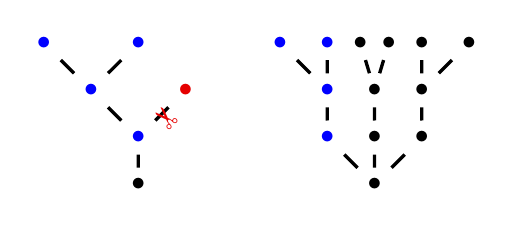
\begin{tikzpicture}[very thick, scale=0.3]
  \node (h1) at (4,0){$\bullet$};
  \node[blue] (h2) at (4,2){$\bullet$};
  \node[blue] (h3) at (2,4){$\bullet$};
  \node[blue] (h4) at (0,6){$\bullet$};
  \node[blue] (h5) at (4,6){$\bullet$};
  \node[red!90!black] (h6) at (6,4){$\bullet$};
  \draw (h1) -- (h2) ;
  \draw (h2) -- (h3) ;
  \draw (h2) -- node[red!90!black,font=\small,sloped,shift={(0.01,-0.075)},rotate=90]{\textbf{\ding{34}}} (h6);
  \draw (h3) -- (h4) ;
  \draw (h3) -- (h5) ;
 
\node (hn1) at (14,0){$\bullet$};
\node[blue] (hn2) at (12,2) {$\bullet$};
\node[blue] (hn3) at (12,4) {$\bullet$};
\node[blue] (hn4) at (10,6){$\bullet$};
  \node[blue] (hn5) at (12,6){$\bullet$};
  \draw (hn1) -- (hn2) ;
  \draw (hn2) -- (hn3) ;
  \draw (hn3) -- (hn4) ;
  \draw (hn3) -- (hn5) ;
\node (hn2b) at (14,2) {$\bullet$};
\node (hn3b) at (14,4) {$\bullet$};
\node (hn4b) at (13.4,6){$\bullet$};
  \node (hn5b) at (14.6,6){$\bullet$};
  \draw (hn1) -- (hn2b) ;
  \draw (hn2b) -- (hn3b) ;
  \draw (hn3b) -- (hn4b) ;
  \draw (hn3b) -- (hn5b) ;
  \node (hn2c) at (16,2) {$\bullet$};
\node (hn3c) at (16,4) {$\bullet$};
\node (hn4c) at (16,6){$\bullet$};
  \node (hn5c) at (18,6){$\bullet$};
  \draw (hn1) -- (hn2c) ;
  \draw (hn2c) -- (hn3c) ;
  \draw (hn3c) -- (hn4c) ;
  \draw (hn3c) -- (hn5c) ;
\end{tikzpicture}

  \caption{Two successive states of a hydra in a battle.  Hercules chopped off the rightmost head of the hydra (red), and the whole left tree except the root node (blue) was copied twice.}
  \label{fig:round}
\end{figure}



 %  \begin{figure}[htb]
% \centering
% \begin{tikzpicture}[very thick, scale=0.3]
% \node (foot) at (10,0) {$\bullet$};
% \node (N1) at (2,2) {$\bullet$};
% \node (N2) at (10,2) {$\bullet$};
% \node (N22) at (7,2) {$\bullet$};
% \node (N3) at (14,2) {$\bullet$};
% \node (N4) at (18,2) {$\Smiley[2][green]$};
% \node (N5) at (0,4) {$\bullet$};
% \node (N6) at (2,5) {$\Smiley[2][green]$};
% \node (N7) at (4,6) {$\Smiley[2][green]$};
% \node (N88) at (7,4) {$\bullet$};
% \node (N8) at (10,4) {$\bullet$};
% \node (N9) at (14,6) {$\Smiley[2][green]$};
% \node (N10) at (0,8) {$\Smiley[2][green]$};
% \node (N11) at (10,7) {$\Smiley[2][green]$};
% \node (N111) at (7,7) {$\Smiley[2][green]$};
% \draw (foot) to [bend left=10] (N1);
% \draw (foot) -- (N2);
% \draw (foot) -- (N22);
% \draw (foot) -- (N3);
% \draw (foot) -- (N4);
% \draw (N1) to  (N5);
% \draw (N1) to   [bend left=10] (N6);
% \draw (N1) to   [bend right=20] (N7);
% \draw (N2) to  (N8);
% \draw (N22) to  (N88);
% \draw (N8) to  (N11);
% \draw (N88) to  (N111);
% \draw (N3) to  (N9);
% \draw (N5) to  (N10);
% \end{tikzpicture}
% \caption{The hydra associated with the ordinal $\omega^{\omega+2}+\omega^\omega \times 2 + \omega + 1$ \label{fig:iota-example}}

% \end{figure}

Kirby and Paris proved the following theorems, applying
combinatorial results about ordinal numbers by Jussi Ketonen and Robert Solovay~\cite{KS81}.

\begin{theorem}
  In the Hydra game, Hercules eventually wins, whichever the strategy of both players:
  choice of a head to chop off, choice of the number of copies.
 \label{kp:thm1}
\end{theorem}

\begin{theorem}
  Theorem~\ref{kp:thm1} cannot be proved in Peano Arithmetic. \label{kp:thm2}
\end{theorem}

The contrast between the simplicity of the statements above and the complexity of their proofs convinced us that it is a good theme for a commented library~\cite{HydraBattles} of formal proofs written for the \coq proof assistant~\cite{Coq}. 

Complex formalizations and proofs are explained in the book.
% an  electronic book~\cite{HydraBook} (PDF document of over 280 pages).
Whenever various reasonable choices exist, we try to present and compare the alternatives.
  For instance, Figures~\ref{fig:Ex42E0} and \ref{fig:Ex42-schutte} show two radically different proofs of the equality
  $\omega+42+\omega^2=\omega^2$. The first one is a simple proof by computation, the second one shows how this equality
  is a consequence of the axioms of the set-theoretic model  by Kurt Schütte~\cite{schutte}. 

This work is also an opportunity to 
 provide concrete examples of formalization and proof techniques: operational type classes, functions defined by  equations, dependently typed functions, etc. It may be also used as a library on ordinal numbers, for instance for proving termination properties.
%
 Prior stages of this project have already been presented at
 JFLA~\cite{PCiota, JFLA2018paper}.
In this paper, we present recent evolutions of the library: new results, interaction with the \community project~\cite{CoqCommunity}, and documentation generated with \alectr~\cite{alectryonpaper, alectryongithub}.

\section{Recent developments}
The 2018 article~\cite{JFLA2018paper} presented a formal proof of the following theorem:

\begin{theorem}
  Let $\mu$ be any ordinal strictly less than $\epsilon_0$.
  There is no function mapping hydras to the segment $[0,\mu)$ that could be used as a measure in proving termination for \emph{any} hydra battle.\label{thm3}
\end{theorem}

Our proof was based on the construction of a battle between Hercules and the hydra where the
number of copies at each round was given by the elimination of an existential quantifier. So, it was mandatory to consider the class of \emph{all} hydra battles, or, equivalently, the class of battles where the hydra choses arbitrarily its number $n$ of copies at every round of the battle.

Unfortunately, the examples  most commonly shown in the literature
(see for instance~\cite{KP82, bauer2008, BauerHydra}) 
assume that the hydra grows $k$ copies at step $k$ of the game, which is incompatible with our proof.
We prove now that Theorem~\ref{thm3} still holds with these typical battles.
%by borrowing new combinatorial results from~\cite{KS81}.
Since we are looking  for a minoration of the length of such battles,
we can work with the following hypotheses and invariants, 
without any loss of generality.
 
 \begin{itemize}
   \item The game starts at an initial step $k=i$, where $i$ is any natural number.
   \item Hercules always chops off the rightmost head of the hydra.
   \item  The hydra is always the tree representation of some ordinal strictly below $\epsilon_0$ in Cantor normal
     form (thus, the rightmost branch is also one of the shortest).
     For instance, Figure~\ref{fig:round} shows the hydras respectively associated with  $\omega^{\omega^2+1}$ and $\omega^{\omega^2}\times 3$.
 \end{itemize}
 
 In mathematical terms, if at step $k\geq i$, the hydra is associated with the ordinal $\alpha$, at step $k+1$ it is associated with
 $\canonseq{\alpha}{k+1}$, \emph{i.e.} the $(k+1)$th element of the canonical sequence of $\alpha$~\cite{KS81}. In the following,  the expression ``the hydra $\alpha$'' is an abbreviation of ``the hydra associated with the ordinal $\alpha$''.
 
 Our new proof of Theorem~\ref{thm3} is based on a systematic study of strictly decreasing sequences of ordinals below $\epsilon_0$, borrowed from Ketonen and Solovay~\cite{KS81}, and the formalization of which is described in detail  in chapters 5 and 6 of~\cite{HydraBook}.

 Besides  Theorem~\ref{thm3}, we study also the number of steps of a battle:
Let $\alpha<\epsilon_0$ be an ordinal. 
We prove that  the number of steps of the battle starting with
$\alpha$ at step $i$ is greater or equal than
$H'_\alpha(i)-i$, where $H'$ is a slight variant of the Hardy hierarchy of rapidly growing functions~\cite{BW85, KS81, Promel2013, Wainer1970}.  The function $H'_\alpha$ is defined by transfinite recursion over $\alpha$ on Figures~\ref{fig:hardy-math}
and~\ref{fig:Hprime}.


\begin{figure}[h]
\begin{align}
  H'_0(i) & = i\\
  H'_\alpha(i) &= H'_{(\canonseq{\alpha}{i+1})}(i)  \quad\textit{if $\alpha$ is a limit ordinal}\\
  H'_{\alpha}(i) &=H'_\beta(i+1) \quad\textit{if $\alpha=\beta+1$}
\end{align}  
  \caption{The $H'$ rapidly growing hierarchy of arithmetical functions}
  \label{fig:hardy-math}
\end{figure}


\begin{figure}[h]
  \centering
  \fbox{
    \begin{minipage}[h]{1.0\linewidth}
 \inputsnippets{Hprime_HprimeDef}     
    \end{minipage}}
 \caption{$H'$ definition with the \texttt{coq-equations}
 plug-in~\cite{sozeau:hal-01671777}}
\label{fig:Hprime}
\end{figure}


Using $H'$s equations as rewrite rules, we can study a concrete example. We take the hydra of figure~\ref{fig:start} and $i=0$ as initial configuration. 
By a sequence of rewritings and inductions, we prove that the number of steps of the considered battle is greater or equal than $2^{2^N}$, where $N=2^{70}-1$.
By comparison with the diagonalized Ackermann function $\lambda\,i.\,A(i,i)$, we prove also that, for $\alpha\geq\omega^\omega$, 
the function computing the length of the battle starting with the hydra $\alpha$ and the initial step $i$ is not primitive recursive.

\begin{figure}[h]
  \centering
  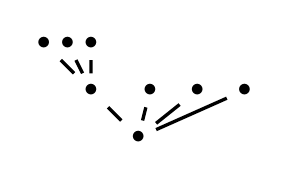
\begin{tikzpicture}[very thick, scale=0.3]
  \node (h1) at (4,0){$\bullet$};
  \node (h2) at (2,2){$\bullet$};
  \node (h3) at (0,4){$\bullet$};
  \node (h4) at (1,4){$\bullet$};
  \node (h5) at (2,4){$\bullet$};
  \node (h6) at (4.5,2){$\bullet$};
  \node (h7) at (6.5,2){$\bullet$};
  \node (h8) at (8.5,2){$\bullet$};
    \draw (h1) -- (h2) ;
    \draw (h2) -- (h3) ;
    \draw (h2) -- (h4) ;
    \draw (h2) -- (h5) ;
    \draw (h1) -- (h6) ;
    \draw (h1) -- (h7) ;
    \draw (h1) -- (h8);
 \end{tikzpicture}

  \caption{The hydra associated with the ordinal $\omega^3+3$}
  \label{fig:start}
\end{figure}




\label{sect:not-pr}

%\TODO[Clément]{Could we use a font with ligatures?}


\section{Integration with \community}

\subsection{Background}

\community is an informal organization run by volunteer Coq users on GitHub that aims to maintain interesting open source Coq projects for the long term and facilitate collaboration among Coq users on documentation, tooling, etc. \community was created in 2018, inspired by the {Elm Community} organization~\cite{zimmermann:tel-02451322}.
%
Such ``Community Package Maintenance Organizations'' exist in many software ecosystems, as they avoid the common problem of an important package becoming unmaintained after its author has moved on to other projects or has disappeared~\cite{zimmermann2021grounded}.

In the case of \coq, this problem is likely even more prevalent than in other ecosystems, as many packages are created by graduate students or researchers for a specific paper and not planned to be maintained for the long term by authors.
%
However, authors are generally open to having someone else who expresses interest in their work take over package maintenance.
%

\community makes it easy to change maintainers by defining a process for transferring or forking an unmaintained package, tooling for setting up good maintenance practices (such as continuous integration), and by making it possible for someone to take over a package without making a long-term commitment (as maintainers who drop out can easily be replaced by some other volunteers).

As of 2021, \community hosts over 50 projects maintained by over 30 volunteers.
%
The hosted projects come from a variety of origins.
%
Some had been maintained in the past by the \coq development team on behalf of the authors, but this meant that only minimal changes required to make the project build with new \coq versions were performed.
%
Some were still maintained by their original authors, but were transferred to enable other users to help out with maintenance and facilitate adoption of best practices on, e.g., continuous integration.
%
Others were simply unmaintained and were revived after their transfer to \community.

Given the objectives of \community, we believe it makes sense to propose a transfer anytime we encounter an interesting Coq project that is insufficiently maintained.
%
After a transfer, the \community maintainers are explicitly allowed to perform large changes and refactorings.
%
This means, for instance, that we can consolidate packages by merging them, or split up a single package into several packages.

\subsection{Integration of primitive recursive functions}

In order to prove formally that the length of the
kind of hydra battles we consider is not given by any primitive recursive function, we chose to use a formalization of primitive recursive functions that was originally part of Russell O'Connor's formal proof of G\"{o}del's first incompleteness theorem~\cite{OConnor05, Goedel}.
For this purpose, and above all in consideration of the scientific interest of this contribution, we decided to host and maintain O'Connor's work in \community.

Since computability is a key topic in computer science teaching and O'Connor's library is a nice illustration of dependently typed programming, we decided to devote a full chapter (chapter 9 of~\cite{HydraBook}) to the formalization of primitive recursive functions, with comments on the definitions and proofs and (counter-)examples and exercises. As part of the writing process, we made the formalization into a new sub-library of the Hydra-battles library, dubbed Ackermann.

\subsection{Towards a bridge to \gaia}

The \gaia project by Jos\'e Grimm aimed to formalize mathematics in \coq in the style of Nicolas Bourbaki. The formalization of the first book in the Elements of Mathematics series by Bourbaki, on the theory of sets, was initially described in a technical report in July 2009~\cite{Grimm2009a}. The set-theoretic axioms and basic definitions in \gaia were derived from an earlier development by Carlos Simpson~\cite{Simpson2004,CatsZFCContrib}. Grimm then wrote (and continually updated) technical reports describing the formalization of Bourbaki's two subsequent books~\cite{Grimm2009b,Grimm2016} and additional topics in number theory~\cite{grimm:hal-00911710,Grimm2014}, before he passed away in 2019.

In 2020, members of \community transferred the \gaia source code to GitHub and adapted it for recent releases of the Mathematical Components library, which \gaia heavily relies on. Anonymous volunteers (``collaborators of Nicolas Bourbaki'') then finished the only in-progress proof left by Grimm. At around 155,000 LOC, \gaia is currently one of the largest maintained open source \coq projects~\cite{Gaia}.

\gaia contains definitions of ordinals in Cantor and Veblen normal form~\cite{grimm:hal-00911710}, adapted from the historical Cantor contribution~\cite{CantorContrib}. The data types for ordinals are essentially defined the same way as in \Hydras, but they are not identical inside \coq, e.g., due to residing in different modules. There are also minor differences in how ordinal arithmetic is implemented, due to the different evolutionary paths taken since divergence from the ancestor library.

As an initial step in bridging \gaia and \Hydras, we were able to establish a correspondence between both implementations of ordinals through rewriting lemmas. For instance, we proved that multiplication of ordinals in Cantor normal form in \Hydras refine \gaia's corresponding multiplication operation, and then imported \gaia's proof of associativity of the multiplication almost for free.

The initial draft bridge code mostly uses the SSReflect proof language and idioms from the Mathematical Components library. We made this design decision since we believe it is less challenging to reason about Hydra-battles code using SSReflect and MathComp than to reason about Gaia without SSReflect.

\subsection{Package Genealogy, Dependencies, and Organization}

Both due to its prior stages~\cite{PCiota,JFLA2018paper} and the recent integrations described just above, the current \Hydras \coq code has a complex inheritance. Figure~\ref{fig:genealogy} illustrates the relationships between \Hydras packages and show their ancestry from historical Coq contributions. To indicate the scope and relative sizes of packages, Table~\ref{tbl:loc} breaks down lines of code for each package in the \Hydras galaxy, as reported by the \texttt{coqwc} tool, and lists their repository names in \community and identifiers in the \coq opam package index~\cite{CoqPackageIndex}.

\begin{figure}[ht]
\centering
{\footnotesize
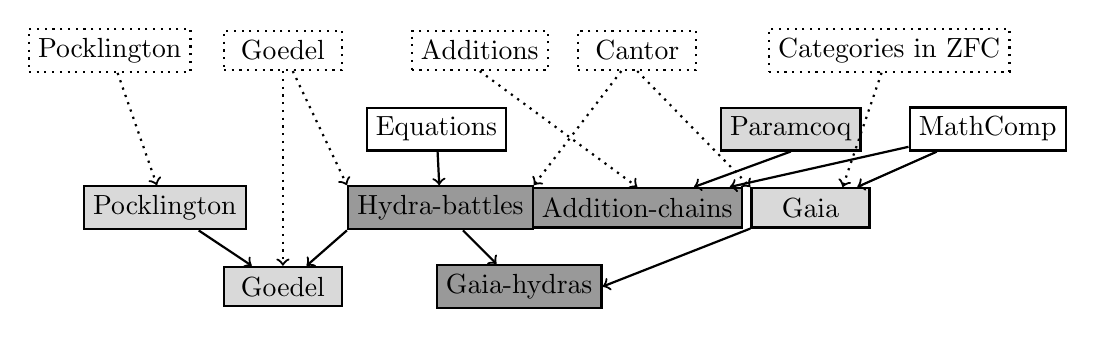
\begin{tikzpicture}[thick]

\begin{scope}[xshift=-6cm]
\node[rectangle, dotted,draw=black,minimum height=0.5cm,minimum width=1.5cm] (goedel) { Goedel };
\node[rectangle, dotted,draw=black,minimum height=0.5cm,minimum width=1.5cm,left of=goedel, node distance=2.2cm] (pock) { Pocklington };
\node[rectangle, dotted,draw=black,minimum height=0.5cm,minimum width=1.5cm,right of=goedel, node distance=2.5cm] (additions) { Additions };
\node[rectangle, dotted,draw=black,minimum height=0.5cm,minimum width=1.5cm,right of=additions, node distance=2cm] (cantor) { Cantor };

\node[rectangle, dotted,draw=black,minimum height=0.5cm,minimum width=1.5cm,right of=cantor, node distance=3.2cm] (cats) { Categories in ZFC };
\end{scope}

\begin{scope}[yshift=-1cm,xshift=0.45cm]
  \node[rectangle, draw=black,fill=gray!30,minimum height=0.5cm,minimum width=1.5cm] (paramcoq) { Paramcoq };
\node[rectangle, draw=black,minimum height=0.5cm,minimum width=1.5cm,right of=paramcoq, node distance=2.5cm] (mathcomp) { MathComp };
\node[rectangle, draw=black,minimum height=0.5cm,minimum width=1.5cm,node distance=2cm,left of=paramcoq, node distance=4.5cm] (equations) { Equations };
\end{scope}

\begin{scope}[yshift=-2cm,xshift=-4cm]
\node[rectangle, draw=black,fill=gray!80,minimum height=0.5cm,minimum width=1.5cm] (hydras) { Hydra-battles };
\node[rectangle, draw=black,fill=gray!30,minimum height=0.5cm,minimum width=1.5cm,left of=hydras, node distance=3.5cm] (pockcc) { Pocklington };
\node[rectangle, draw=black,fill=gray!80,minimum height=0.5cm,minimum width=1.5cm,right of=hydras, node distance=2.5cm] (chains) { Addition-chains };
\node[rectangle, draw=black,fill=gray!30,minimum height=0.5cm,minimum width=1.5cm,right of=chains, node distance=2.2cm] (gaia) { Gaia };
\end{scope}

\begin{scope}[yshift=-3cm,xshift=-6cm]
 \node[rectangle, draw=black,fill=gray!30,minimum height=0.5cm,minimum width=1.5cm] (goedelcc) { Goedel };
 \node[rectangle, draw=black,fill=gray!80,minimum height=0.5cm,minimum width=1.5cm,right of=goedelcc, node distance=3cm] (gaiahydras) { Gaia-hydras };
\end{scope}

\draw[->,dotted] (additions.south) -- (chains.north) ;
\draw[->,dotted] (goedel) -- (goedelcc) ;
\draw[->,dotted] (goedel) -- (hydras.north west) ;
\draw[->,dotted] (cantor) -- (hydras.north east) ;
\draw[->,dotted] (cantor.south) -- (gaia.north west) ;
\draw[->,dotted] (pock) -- (pockcc) ;
\draw[->,dotted] ([xshift=2.1cm]cats) -- (gaia) ;

\draw[->] (hydras) -- (gaiahydras) ;
\draw[->] (hydras.south west) -- (goedelcc) ;
\draw[->] (gaia.south west) -- (gaiahydras.east) ;

\draw[->] (equations) -- (hydras) ;
\draw[->] (mathcomp) -- (gaia) ;
\draw[->] (mathcomp) -- (chains) ;
\draw[->] (paramcoq.south) -- (chains) ;
\draw[->] (pockcc) -- (goedelcc) ;
\end{tikzpicture}
}
\caption{Genealogy and dependencies for \Hydras packages. Dotted boxes represent historical Coq contributions, while regular boxes represent maintained \coq packages. Dark gray packages are maintained in the \Hydras GitHub repository, while light gray packages are maintained in other \community repositories. Dotted lines represent \coq code ancestry, while regular lines represent direct code dependencies.}
  \label{fig:genealogy}
\end{figure}

Before the Ackermann sub-library was moved from the Goedel package repository to the \Hydras repository, the Goedel package had around 7,000 specification LOC and 38,000 proof LOC. Figure~\ref{fig:genealogy} and Table~\ref{tbl:loc} thus reveal that the seemingly large Coq formalization of G\"{o}del's incompleteness theorem can be viewed as a modestly-sized proof on top of general libraries for, on the one hand, first-order logic, primitive recursive functions, and Peano Arithmetic (Ackermann), and on the other hand, prime numbers and their properties (Pocklington).

\begin{table}[ht]
\centering
\footnotesize
\begin{tabular}{llllrr}
\hline
\textbf{Package name} & \textbf{Repository} & \textbf{Index identifier} & \textbf{Version} & \textbf{Spec LOC} & \textbf{Proof LOC}\\
\hline
Pocklington & \href{https://github.com/coq-community/pocklington}{\texttt{pocklington}} & \texttt{coq-pocklington} & \texttt{8.12.0} & 825 & 3,798 \\
Goedel & \href{https://github.com/coq-community/goedel}{\texttt{goedel}} & \texttt{coq-goedel} & \texttt{8.13.0} & 2,799 & 10,762 \\
Gaia & \href{https://github.com/coq-community/gaia}{\texttt{gaia}} & \texttt{coq-gaia} & \texttt{1.12} & 28,850 & 124,839 \\
Hydra-battles & \href{https://github.com/coq-community/hydra-battles}{\texttt{hydra-battles}} & \texttt{coq-hydra-battles} & \texttt{0.5} & 14,368 & 48,385 \\
Addition-chains & \href{https://github.com/coq-community/hydra-battles}{\texttt{hydra-battles}} & \texttt{coq-addition-chains} & \texttt{0.5} & 1,961 & 2,210 \\
Gaia-hydras & \href{https://github.com/coq-community/hydra-battles}{\texttt{hydra-battles}} & \texttt{coq-gaia-hydras} & \texttt{0.5} & 81 & 177 \\
\hline
\end{tabular}
\caption{Current numbers of lines of code for packages in the \Hydras galaxy.}
\label{tbl:loc}
\end{table}

In traditional software development, it is common for packages to continually depend on a large number of packages. In contrast, projects in the Coq ecosystem are often subject to ``dependency aversion'', where maintainers eschew depending on useful packages because it may lead to work in adapting to upstream changes. With \Hydras, we hope to demonstrate that projects with complex dependencies are feasible to manage using recent advances in build management and infrastructure.

% We could already talk a bit of the monorepo structure here, and
% defer some explanations on the tooling to the next section.

\section{Modernizing the build infrastructure}

\subsection{Documentation with \alectr}

The \Hydras book is written in LaTeX, but it makes very frequent references (about once per page, 274 snippets over 281 pages) to parts of the \coq development, showing definitions (Fig.~\ref{fig:Hprime}), computation results (Fig.~\ref{fig:Pow-evalPow17LetIn}), lemmas (Fig.~\ref{fig:Ex42E0}) and parts of  proof scripts (Fig.~\ref{fig:Ex42-schutte}). The order in which these references appear in the book is independent of the structure of our libraries, so we chose to maintain the book as a standalone document, separate from the \coq source code.  This contrasts with the \coqdoc approach, where explanatory prose is embedded within \coq source files (a detailed discussion of different approaches to documenting \coq developments can be found in \cite{alectryonpaper}).

Originally, we copied snippets from \coq sources into LaTeX manually, and recorded and inserted the corresponding outputs manually as well.  This approach is common, but brittle: changes to \coq definitions or lemmas had to be reflected in the book's sources, and we found multiple instances where the book and the \coq development had diverged.
 
We solved this maintenance issue by moving to \alectr, a tool that automatically records \coq proofs~\cite{alectryongithub}.  Instead of copy-pasting fragments into LaTeX, we now embed small LaTeX files automatically generated by \alectr from our \coq development.  Our build system guarantees that these LaTeX snippets are always up-to-date and consistent with the code (and, by comparing these snippets across releases of \coq or versions of \Hydras, we can easily spot unexpected changes).

Importing snippets into a LaTeX document was not one of the original use cases of Alectryon. Firstly, the original Alectryon did not have support for exporting to LaTeX. Secondly, it was geared towards documenting individual source files, where code and prose are interleaved within the same file. In this style, the code is documented in the same order as it is compiled.
We extended \alectr to support our needs by implementing a LaTeX backend, and by programming it to generate individual snippet files, one per \texttt{snippet} comment block.  The later part was straightforward: all it took was to build a custom \alectr \textit{driver}, a small (about 100 lines) Python program that leverages most of the \alectr toolchain but defines a custom frontend that understands our snippet annotations (and otherwise exposes the exact same command line as \alectr).

Once the infrastructure was in place, the transition happened gradually, over a few weeks: for each snippet of \coq code that was in the book, we had to take the following steps:

\begin{enumerate}
\item Mark the snippet in the \coq sources (we use special comments \texttt{(* begin snippet \textit{name} *)} … \texttt{(* end snippet \textit{name} *)})
\item Configure output display, using special \alectr annotations to configure what should be shown (only the inputs, inputs and outputs, some steps of the proof but not all, some proof states at key moments in a proof, etc.)
\item Replace the copy-pasted inputs and output in LaTeX with an \texttt{input} command.
\end{enumerate}

   \begin{figure}[h]
     \centering
     \fbox{
       \begin{minipage}[h]{1.0\linewidth}
         \inputsnippets{Pow_evalPow17LetIn}
       \end{minipage}}
  \caption{\label{fig:Pow-evalPow17LetIn}Automatically capturing the output of computations}
\end{figure}


  \begin{figure}[h]
    \centering
    \fbox{
      \begin{minipage}[h]{1.0\linewidth}
        \inputsnippets{E0_Ex42}
      \end{minipage}}
    \caption{A simple proof by computation}
    \label{fig:Ex42E0}
  \end{figure}



%\afterpage{\clearpage}

 


\begin{figure}[th]
  \centering
  
  

\fbox{\begin{minipage}[h]{1.0\linewidth}
  Let us prove again the equality $\omega+42+\omega^2= \omega^2$. We recall that $\omega^2$ is an abbreviation of $\phi_0(2)$,
\emph{i.e} the third  additive principal ordinal, and that \texttt{F} is a notation for the coercion which maps natural numbers to ordinals.

\inputsnippets{Schutte_Ex42a}


Our proof is very different from the computational proof of
Figure~\ref{fig:Ex42E0}.
By definition of additive principal ordinals, 
it suffices to prove the inequality $\omega+42< \phi_0(2)$.

\inputsnippets{Schutte_Ex42b}

Since the set \textit{AP} of additive principals  is closed under addition
(by Lemma \textit{AP\_plus\_closed}), it suffices to prove the inequalities $\omega<\omega^2$ and $42<\omega^2$.

\inputsnippets{Schutte_Ex42d, %to remove if short paper
  Schutte_Ex42c, Schutte_Ex42e}

\end{minipage}
}
\caption{A proof interleaved with text (from the book)}
  \label{fig:Ex42-schutte}
\end{figure}

\paragraph{Applications in other proof assistants.}
The Alectryon toolchain is intended to eventually support the languages of many proof assistants, and already has preliminary support for Lean~3. Our Alectryon extensions for snippet generation are in principle applicable to any language supported by Alectryon. However, snippet delimiters are language specific, and our tooling currently assumes Coq-compatible delimiters; we expect to lift this restriction in the near future. We view \Hydras as an incubator for experimental Alectryon features that, when deemed stable and useful, can be disseminated to a wider audience including users of other proof assistants.

\subsection{Technologies supporting the monorepo structure}

A monorepo (shorthand for monolithic repository) is a version control repository containing multiple independent or related packages.
%
Monorepos have gained increasing popularity following experiences in large companies such as Google, but are also used at a smaller scale for managing open source projects.
%
They are known to simplify the management of dependencies, making cross-packages changes, and refactorings~\cite{brito2018monorepos}.

%
One of the few early uses of monorepos in the Coq ecosystem was for the Mathematical Components library~\cite{MCB}, whose maintainers developed a custom build infrastructure to check multiple packages on each commit.
%
In light of that recent tooling improvements have made monorepo use easier, we chose to use an explicit monorepo structure for \Hydras in \community. Other \community projects have since adopted a similar structure.

In the context of \Hydras, we rely on the following tools.

\paragraph{The Dune build system~\cite{dune}.}
Dune was originally designed to build OCaml projects, but was recently extended to support Coq. Dune allows building packages contained in a single source tree separately, which is essential to be able to publish the different libraries contained in a single repository as separate (opam) packages to the Coq package index.

However, Dune is currently inconvenient for local IDE-based Coq code development and does not yet support building \coqdoc files.
%
Therefore, we still support building the whole project using \make via the \coqmakefile tool bundled with \coq, and we rely on this build system in our documentation generation pipeline.
%
We expect to migrate fully to Dune as soon as these limitations are lifted.

\paragraph{Docker-Coq-Action~\cite{martindorel2020dockercoq}.}
This GitHub Action provides a very simple way of setting up Continuous Integration (CI) for a Coq project with an opam file.
%
At the current time, we rely on it, together with the mathcomp Docker images~\cite{mathcompdocker}, to test our two main libraries, Hydra-battles and Addition-chains, with multiple versions of Coq.

\paragraph{The Coq Nix Toolbox~\cite{cohen:hal-03366644}.}
This toolbox, based on the Nix package manager, provides an alternative way of setting up CI for a Coq project (also relying on GitHub Actions).
%
We use this Nix-based CI for several things.

\begin{enumerate}
\item To test the build of the project (as a single unit) with \coqmakefile (whereas the Docker-based CI relies on the opam packages, which use Dune to build the libraries contained in the project).

\item To generate the documentation of the project (book in PDF format and \coqdoc HTML pages) by relying on the output of the \coqmakefile build.

\item To test the bridge to the Gaia library, because the Nix-based CI supports out-of-the-box caching of build dependencies.
%
Given that Gaia takes more than 5 minutes to build, this build is only done once, then reused at each new run of the CI.

\item To test compatibility with the Goedel library, which was made to depend on the Hydra-battles library since the Ackermann sub-library was moved from the former to the latter.
%
For this, we rely on the fact that the Coq Nix Toolbox has native support for generating a CI configuration that includes reverse dependency compatibility testing.
\end{enumerate}

The artifacts of the Nix builds are stored in the \community binary cache on Cachix~\cite{cachix}.
%
This means that a given version never has to be built twice and Continuous Integration can be almost instantaneous when no change has been made (e.g., after merging a pull request).

By relying on two different technologies for CI, we are able to fit a larger range of use cases, while also providing more assurance that the project does build correctly in a variety of configurations.
%
Given that the two technologies are well maintained (within \community), relying on both does not incur a significant cost, compared to the benefits they provide.

\section{Comparison of \Hydras with other Coq books}

We believe that Coq books can broadly be divided into two categories:
\begin{itemize}
\item \emph{Executable textbooks} that are in effect large, well-commented Coq programs from which other representations of the material (HTML, PDF) are derived using tools.
\item \emph{Traditional textbooks} generated from documentation languages such as LaTeX that are accompanied by standalone Coq formalizations and/or code snippets.
\end{itemize}
Table~\ref{tbl:books} shows a category breakdown for what we believe are the most prominent Coq books in English. Note that several traditional books, such as Coq'Art~\cite{BC04}, used custom tools during their writing process to keep code snippets synchronized with Coq. However, once a book is published, the accompanying code generally takes on a life of its own~\cite{CoqArtCommunity} and may come to substantially diverge from the book.

\begin{table}
  \centering
  \footnotesize
  \begin{tabular}{lll}
  \hline
  \textbf{Title} & \textbf{Year} & \textbf{Category}\\
  \hline
  Coq'Art~\cite{BC04} & 2004 & Traditional\\
  Software Foundations~\cite{SF} & 2007 & Executable\\
  Certified Programming with Dependent Types~\cite{chlipalacpdt2011} & 2011 &  Executable\\
  Program Logics for Certified Compilers~\cite{Appel2014} & 2014 & Traditional\\
  Programs and Proofs~\cite{Sergey:PnP} & 2014 & Executable\\
  Formal Reasoning About Programs~\cite{Chlipala2017} & 2017 & Traditional\\
  Computer Arithmetic and Formal Proofs~\cite{Boldo2017} & 2017 & Traditional\\
  Mathematical Components~\cite{MCB} & 2018 & Traditional\\
  \hline
  \end{tabular}
  \caption{Coq book categorization.}
  \label{tbl:books}
\end{table}

We believe the \Hydras electronic book has found an attractive set of tradeoffs between the properties of executable books and traditional books. Specifically, in an executable book, the proof assistant language places limits on the structure. For example, Coq may not permit repeating a definition from another file verbatim, since the definition uses variables that are not present in the current context. Thanks to our \alectr based toolchain, the \Hydras book can include ``live'' code fragments at any point in the text. And in contrast to traditional books, we validate the consistency of code fragments during every build of the electronic book. On the one hand, we follow executable books in providing ``continuous delivery'' of new revisions at a high pace. But on the other hand, we also aim to make regular timestamped versions compatible with specific versions of Coq, akin to new editions of traditional books.

Due to our reliance on LaTeX for writing the book, obtaining a book representation in HTML is more cumbersome than for executable books such as Software Foundations~\cite{SF} and Certified Programming with Dependent Types~\cite{chlipalacpdt2011}. Currently, we generate the Coq code documentation in HTML form separately from the book.

\section{Conclusion and perspectives}


\Hydras wants to provide a connection between scientific literature (\emph{e.g.},~\cite{KP82, KS81, schutte}) and proof assistant technology. For the mathematician, it can give a concrete view of the mathematical content, not only through full proofs, but also through illuminating computations: examples, functions associated with constructive proofs, etc. For the \coq learner, it provides a consistent set of examples,
allowing to present and compare various formalization and proving techniques. %It may be also used as a library, through opam packages.
It is also a medium sized library (more than 50,000 LOC), dependent on various tools and libraries of the \coq ecosystem, which may be also used to experiment with new maintenance techniques of the code and its documentation. To facilitate easy dissemination and reuse, all code and documentation is available under the permissive MIT license.





%\TODO{General Conclusion}



%\subsection{Perspectives}

%\subsection{Further extensions}

We plan to extend \Hydras in two main directions. Firstly, we plan to bridge the combinatorial results of \Hydras and the set-theoretic content of \gaia, enabling the transfer of many interesting theorems between the two packages. Secondly, we aim to write a formal proof in \coq of the original statement of Theorem~\ref{kp:thm2}, using O'Connor's formalization of Peano Arithmetic~\cite{Goedel}.
%
Moreover, \Hydras is not limited to the study of ordinal numbers and applications.
We are also developing a package about efficient exponentiation
algorithms, and aim to eventually include new topics. We invite new collaborators to join us in our efforts.

\section*{Acknowledgments}
\label{sect:acks}
We thank the anonymous reviewers for their comments, and we are grateful to the original authors and current maintainers of the Coq packages we use and depend on: José Grimm (Gaia), Russell O'Connor (Goedel), Matthieu Sozeau (Equations), the Mathematical Components team, Marc Lasson and Chantal Keller (Paramcoq), and the authors and maintainers of \coq and its associated tools.


\label{sect:bib}
\bibliographystyle{plain}
%\bibliographystyle{alpha}
%\bibliographystyle{unsrt}
%\bibliographystyle{abbrv}
\input{paper.bbl}

%\bibliography{../thebib}


\end{document}



%\bibliography{../thebib}


\end{document}



%\bibliography{../thebib}


\end{document}



%\bibliography{../thebib}


\end{document}

